% Options for packages loaded elsewhere
\PassOptionsToPackage{unicode}{hyperref}
\PassOptionsToPackage{hyphens}{url}
%
\documentclass[
  12pt,
]{article}
\usepackage{amsmath,amssymb}
\usepackage{iftex}
\ifPDFTeX
  \usepackage[T1]{fontenc}
  \usepackage[utf8]{inputenc}
  \usepackage{textcomp} % provide euro and other symbols
\else % if luatex or xetex
  \usepackage{unicode-math} % this also loads fontspec
  \defaultfontfeatures{Scale=MatchLowercase}
  \defaultfontfeatures[\rmfamily]{Ligatures=TeX,Scale=1}
\fi
\usepackage{lmodern}
\ifPDFTeX\else
  % xetex/luatex font selection
\fi
% Use upquote if available, for straight quotes in verbatim environments
\IfFileExists{upquote.sty}{\usepackage{upquote}}{}
\IfFileExists{microtype.sty}{% use microtype if available
  \usepackage[]{microtype}
  \UseMicrotypeSet[protrusion]{basicmath} % disable protrusion for tt fonts
}{}
\usepackage{xcolor}
\usepackage[margin=1in]{geometry}
\usepackage{longtable,booktabs,array}
\usepackage{calc} % for calculating minipage widths
% Correct order of tables after \paragraph or \subparagraph
\usepackage{etoolbox}
\makeatletter
\patchcmd\longtable{\par}{\if@noskipsec\mbox{}\fi\par}{}{}
\makeatother
% Allow footnotes in longtable head/foot
\IfFileExists{footnotehyper.sty}{\usepackage{footnotehyper}}{\usepackage{footnote}}
\makesavenoteenv{longtable}
\usepackage{graphicx}
\makeatletter
\def\maxwidth{\ifdim\Gin@nat@width>\linewidth\linewidth\else\Gin@nat@width\fi}
\def\maxheight{\ifdim\Gin@nat@height>\textheight\textheight\else\Gin@nat@height\fi}
\makeatother
% Scale images if necessary, so that they will not overflow the page
% margins by default, and it is still possible to overwrite the defaults
% using explicit options in \includegraphics[width, height, ...]{}
\setkeys{Gin}{width=\maxwidth,height=\maxheight,keepaspectratio}
% Set default figure placement to htbp
\makeatletter
\def\fps@figure{htbp}
\makeatother
\setlength{\emergencystretch}{3em} % prevent overfull lines
\providecommand{\tightlist}{%
  \setlength{\itemsep}{0pt}\setlength{\parskip}{0pt}}
\setcounter{secnumdepth}{-\maxdimen} % remove section numbering
% definitions for citeproc citations
\NewDocumentCommand\citeproctext{}{}
\NewDocumentCommand\citeproc{mm}{%
  \begingroup\def\citeproctext{#2}\cite{#1}\endgroup}
\makeatletter
 % allow citations to break across lines
 \let\@cite@ofmt\@firstofone
 % avoid brackets around text for \cite:
 \def\@biblabel#1{}
 \def\@cite#1#2{{#1\if@tempswa , #2\fi}}
\makeatother
\newlength{\cslhangindent}
\setlength{\cslhangindent}{1.5em}
\newlength{\csllabelwidth}
\setlength{\csllabelwidth}{3em}
\newenvironment{CSLReferences}[2] % #1 hanging-indent, #2 entry-spacing
 {\begin{list}{}{%
  \setlength{\itemindent}{0pt}
  \setlength{\leftmargin}{0pt}
  \setlength{\parsep}{0pt}
  % turn on hanging indent if param 1 is 1
  \ifodd #1
   \setlength{\leftmargin}{\cslhangindent}
   \setlength{\itemindent}{-1\cslhangindent}
  \fi
  % set entry spacing
  \setlength{\itemsep}{#2\baselineskip}}}
 {\end{list}}
\usepackage{calc}
\newcommand{\CSLBlock}[1]{\hfill\break\parbox[t]{\linewidth}{\strut\ignorespaces#1\strut}}
\newcommand{\CSLLeftMargin}[1]{\parbox[t]{\csllabelwidth}{\strut#1\strut}}
\newcommand{\CSLRightInline}[1]{\parbox[t]{\linewidth - \csllabelwidth}{\strut#1\strut}}
\newcommand{\CSLIndent}[1]{\hspace{\cslhangindent}#1}
\usepackage{setspace}\doublespacing
\usepackage{indentfirst}
\usepackage[small]{titlesec}
\usepackage{wrapfig}
\usepackage{caption}
\captionsetup[figure]{font={scriptsize, doublespacing}, labelfont=bf, aboveskip=4pt, belowskip=-15pt}
\usepackage{hanging}
\usepackage[left]{lineno}
\usepackage{booktabs}
\usepackage{longtable}
\usepackage{array}
\usepackage{multirow}
\usepackage{wrapfig}
\usepackage{float}
\usepackage{colortbl}
\usepackage{pdflscape}
\usepackage{tabu}
\usepackage{threeparttable}
\usepackage{threeparttablex}
\usepackage[normalem]{ulem}
\usepackage{makecell}
\usepackage{xcolor}
\ifLuaTeX
  \usepackage{selnolig}  % disable illegal ligatures
\fi
\usepackage{bookmark}
\IfFileExists{xurl.sty}{\usepackage{xurl}}{} % add URL line breaks if available
\urlstyle{same}
\hypersetup{
  pdftitle={How resource abundance and resource stochasticity affect organisms' range sizes},
  pdfauthor={Stefano Mezzini1,2; Chris H. Fleming3,4; E. Patrícia Medici5,6,7; Michael J. Noonan1,2,8,},
  hidelinks,
  pdfcreator={LaTeX via pandoc}}

\title{\large How resource abundance and resource stochasticity affect organisms' range sizes}
\author{Stefano Mezzini\textsuperscript{1,2} \and Chris H. Fleming\textsuperscript{3,4} \and E. Patrícia Medici\textsuperscript{5,6,7} \and Michael J. Noonan\textsuperscript{1,2,8,*}}
\date{}

\begin{document}
\maketitle

\textsuperscript{1} Okanagan Institute for Biodiversity, Resilience, and Ecosystem Services, The University of British Columbia Okanagan, Kelowna, British Columbia, Canada.\\
\textsuperscript{2} Department of Biology, The University of British Columbia Okanagan, Kelowna, British Columbia, Canada.\\
\textsuperscript{3} Department of Biology, University of Central Florida, Orlando, Florida 32816, United States.\\
\textsuperscript{4} Smithsonian Conservation Biology Institute, National Zoological Park, 1500 Remount Rd., Front Royal, VA 22630, United States.\\
\textsuperscript{5} Lowland Tapir Conservation Initiative (LTCI), Instituto de Pesquisas Ecológicas (IPÊ), Rodovia Dom Pedro I, km 47, Nazaré Paulista, São Paulo 12960-000, Brazil.\\
\textsuperscript{6} IUCN SSC Tapir Specialist Group (TSG), Campo Grande, Brazil.\\
\textsuperscript{7} Escola Superior de Conservação Ambiental E Sustentabilidade (ESCAS/IPÊ), Rodovia Dom Pedro I, km 47, Nazaré Paulista, São Paulo 12960-000, Brazil.\\
\textsuperscript{8} Department of Computer Science, Math, Physics, and Statistics, The University of British Columbia Okanagan, Kelowna, British Columbia, Canada.

\textsuperscript{*} Correspondence: \href{mailto:michael.noonan@ubc.ca}{Michael J. Noonan \textless{}\href{mailto:michael.noonan@ubc.ca}{\nolinkurl{michael.noonan@ubc.ca}}\textgreater{}}

\newcommand*\e{\text{E}}

\newcommand*\var{\text{Var}}

\clearpage

\noindent \textbf{Article type}: Research article

\noindent \textbf{Words in abstract}: 274

\noindent \textbf{Words in main text}: 6722

\noindent \textbf{Figures}: 6

\noindent \textbf{Tables}: 0

\noindent \textbf{References}: 112

\noindent \textbf{Appendices}: 3

\noindent \textbf{Key words:} energetics, resource abundance, resource stochasticity, environmental stochasticity, home range, range size, movement behavior, \texttt{ctmm}

\newpage

\doublespacing

\linenumbers

\section{Abstract}\label{abstract}

\noindent \textbf{Background:} From megafauna to amoebas, the amount of space heterotrophic organisms use is thought to be tightly linked to the availability of resources within their habitats, such that organisms living in productive habitats generally require less space than those in resource-poor habitats. This hypothesis has widespread empirical support, but existing studies have focused primarily on responses to spatiotemporal changes in mean resources, while responses to unpredictable changes in resources (i.e., variance in resources or resource stochasticity) are still largely unknown. Since organisms adjust to variable environmental conditions, failing to consider the effects of resource unpredictability can result in an insufficient understanding of an organism's range size. \textbf{Methods:} We leverage the available literature to provide a unifying framework and hypothesis for the effects of resource abundance and stochasticity on organisms' range sizes. We then use simulated movement data to demonstrate how the combined effects of resource abundance and stochasticity interact to shape predictable patterns in range size. Finally, we test the hypothesis using real-world tracking data on a lowland tapir (\emph{Tapirus terrestris}) from the Brazilian Cerrado. \textbf{Results:} Organisms' range sizes decrease nonlinearly with resource abundance and increase nonlinearly with resource stochasticity, and the effects of resource stochasticity depend strongly on resource abundance. Additionally, the distribution and predictability of resources can exacerbate the effects of other drivers of movement, such as resource depletion, competition, and predation. \textbf{Conclusions:} Accounting for resource abundance and stochasticity is crucial for understanding the movement behavior of free-ranging organisms. Failing to account for resource stochasticity can lead to an incomplete and incorrect understanding of how and why organisms move, particularly during periods of rapid change.

\newpage

\section{Background}\label{background}

\noindent The amount of resources an organism is able to access is a strong determinant of its fitness. Resource limitations can cause individuals to experience a negative energetic balance, which can then result in lower fitness {[}1,2{]}, altered physiology {[}2--5{]}, lower chance of reproduction {[}2,6--8{]}, and even death {[}9,10{]}. Thus, many organisms adapt their behaviors and/or physiology in response to changes in local resource abundance to ensure their needs are met {[}e.g., soil amoebae \emph{Dictyostelium spp.}: 11,plants: 12,and animals: 13{]}.

While there are many ways that individuals can respond to resource availability, movement represents one of the most readily available traits that motile species can adjust {[}14--16{]}. The relationship between organisms' movement and resource abundance has long been of interest to biologists. In his seminal paper, Burt {[}17{]} considered the search for food as the primary driver for movement within an organism's home range. Three decades after, Southwood {[}18{]} suggested that change in resource abundance drives how organisms decide where to live and when to reproduce. Two years later, Harestad and Bunnel {[}13{]} proposed that the simplest relationship between resource abundance and an organism's home-range size is

\begin{equation}
H = C / R,
\label{eq:harestad-eq}
\end{equation}

\noindent where \(H\) is the organism's home-range size, \(C\) is the organism's resource consumption rate (kcal day\(^{-1}\)), and \(R\) is the resources the organism can access (kcal day\(^{-1}\) unit area\(^{-1}\)). Harestad and Bunnel's model is simple to conceptualize, and it allows for testable predictions, but few studies are structured around a set of theoretical expectations such as Harestad and Bunnel's hypothesis. Many researchers have since demonstrated that organisms adapt their range sizes in response to resource abundance, but results are typically reported as independent, novel findings. Perhaps more problematic is the fact that, while much work has been done on estimating organisms' responses to changes in mean resource abundance, there is little information on how organisms respond to unpredictable changes in resources {[}i.e., resource stochasticity, but see: 19,20--22{]}. Thus, there remains a need for a clear, unifying hypothesis of the effects of both resource abundance and stochasticity on organisms' range sizes.

Here, we refer to a location's average amount of resources as ``resource abundance'', while we use the phrase ``resource stochasticity'' to indicate the variability in resources after accounting for changes in the mean. We argue that, on its own, a habitat's resource abundance is not sufficient to assess the habitat's quality, nor make predictions about how much space an organism might use. To see this, consider, for instance, a herbivore grazing in a grassland with relatively low but constant forage availability (i.e., low mean and variance). The animal may require a large but constant home range size as it moves between patches in search of food. If, instead, it lived in a desert with equally scarce forage but rare, sudden, and strong pulses of resources (i.e., low long-term mean and high stochasticity), it may switch between dispersal in search for high-resource patches and short-term range residency within patches {[}\emph{sensu} 15,see 23,24,25{]}. Previous studies suggest that resource stochasticity may decrease organisms' fitness and landscapes' energetic balances {[}e.g., 26{]}, but there is still limited empirical evidence to support this hypothesis {[}but see: 21,27,28{]}.

In this paper, we illustrate how an organism's range size can be expected to depend on both the abundance and unpredictability of resources. First, we set the theoretical background necessary for the successive sections by introducing key concepts and notation. Next, we provide a review of the effects of resource abundance on range sizes while suggesting a simple and unifying hypothesis. Afterwards, we provide a review of the effects of resource stochasticity on organisms' range sizes while suggesting a second simple and unifying hypothesis. Subsequently, we support the hypothesis using quantitative, simulated responses in range size to changes in resource abundance and stochasticity. Finally, we demonstrate how this framework can be used in practice to describe the movement ecology of a lowland tapir (\emph{Tapirus terrestris}) from the Brazilian Cerrado {[}29{]}.

\section{Resources as a random variable}\label{resources-as-a-random-variable}

\noindent Resources (e.g., food, water, shelter, heat) are often unpredictable (and difficult to quantify), since they depend on various factors which cannot be accounted for easily, including climate {[}7,30,31{]}, weather {[}31,32{]}, competitive pressure {[}33,34{]}, and differences in energetics at among individuals {[}7{]} and species {[}35{]}. Thus, it is possible to treat the amount of resources \(R\) at a given point in time (\(t\)) and space (location vector \(\vec u\)) as a random variable, denoted as \(R(t, \vec u)\). Treating resources as a random variable allows us to leverage techniques from probability theory and statistics, such as the expectation of a random variable (i.e., its mean) and its variance around the mean. We indicate the expected value and variance of random variable \(R\) using \(\text{E}(R)\) and \(\text{Var}(R)\), respectively, and we use \(\mu(t, \vec u)\) and \(\sigma^2(t, \vec u)\) to indicate them as functions of time (\(t\)) and space (\(\vec u\)). Appendix A defines and expands on the concepts of probability distributions, expected value, variance, and provides examples of them for Gamma and Beta distributions.

\subsection{\texorpdfstring{Effects of resource abundance, \(\text{E}(R)\)}{Effects of resource abundance, \textbackslash text\{E\}(R)}}\label{effects-of-resource-abundance-texter}

\noindent While organisms' needs vary greatly between taxonomic groups, some needs are essential for the growth, survival, and reproduction of most organisms. All heterotrophic organisms require sources of chemical energy (i.e., food), water, and various limiting nutrients {[}36--38{]}. As the abundance of essential resources fluctuates, motile organisms can move to new locations or `patches' to meet their requirements {[}15,39{]}, but movement also increases energetic needs {[}40{]}.

When \(\text{E}(R)\) is high, we expect organisms' ranges to be relatively small and near the smallest amount of space required to survive {[}see fig.~\ref{fig:hr-hyp}A as well as: 27,28,41{]}. Like Harestad and Bunnel {[}13{]}, we also expect organisms' range sizes to increase nonlinearly as \(\text{E}(R)\) decreases, but we highlight that organisms may adopt different behaviors at low values of \(\text{E}(R)\). These behaviors include maximal home range expansion {[}home range size is limited by vagility, habitat structure, competition, and predation, e.g., 33,34,42,43{]}, migration {[}44--46{]}, and nomadism {[}23,25,47,48{]}. It is unclear when organisms switch from range residency to migration or nomadism (or vice-versa), but understanding the gradient among these types of movement is necessary for quantifying the effect of resource abundance on organisms' range size and movement behavior {[}mammals: 49,moose, \emph{Alces alces}: 23,eagles, \emph{Haliaeetus leucocephalus}: 24,50,lesser flamingos, \emph{Phoeniconaias minor}: 51{]}.

\begin{figure}

{\centering \includegraphics[width=\textwidth]{../figures/hr-hypotheses} 

}

\caption{Hypothesized range size of an organism as a function of (A) resource abundance and (B) resource stochasticity. We expect low values of $\text{E}(R)$ and large values of $\text{Var}(R)$ to result in a large range, since organisms are forced to explore large areas to collect the resources they require to survive, whether they be range-resident, nomadic, or migratory. As $\text{E}(R)$ increases or $\text{Var}(R)$ decreases, range size should decrease nonlinearly until it reaches the minimum amount of space required by the organism to survive.\\Note that the relationship between range size and both $\text{E}(R)$ and $\text{Var}(R)$ cannot be of the form $H = \beta_0 + \beta_1 \text{E}(R) + \beta_2 \text{Var}(R)$ because it would require range size to be negative for high values of $\text{E}(R)$ or low values of $\text{Var}(R)$.}\label{fig:hr-hyp}
\end{figure}

Overall, the hypothesis that range size decreases with resource abundance, \(\text{E}(R)\), is commonly accepted and well supported, but many studies assume a linear relationship {[}e.g., 21,41,52--54{]}. This is problematic because, conceptually, the relationship between range size and \(\text{E}(R)\) must be nonlinear, since: (1) there is an upper limit to how much space an organism is able to explore in its finite lifetime and (2) the minimum amount of space it requires to survive is necessarily greater than zero {[}see 27,28,55,56,57, and contrast them to the earlier references that assume a linear relationship between \(H\) and \(R\){]}. Consequently, we suggest analysts use models that account for this nonlinearity when estimating the effects of resource abundance on range size. While the relationship may be approximately linear for some range of \(\text{E}(R)\), this assumption often does not hold for low or high values of \(\text{E}(R)\) {[}e.g., 52{]}. Additionally, identifying inflection points in nonlinear relationships can help understand the pressures and limitations of increasing range size.

\subsection{\texorpdfstring{Effects of resource stochasticity, \(\text{Var}(R)\)}{Effects of resource stochasticity, \textbackslash text\{Var\}(R)}}\label{effects-of-resource-stochasticity-textvarr}

\noindent Assuming resource stochasticity is constant over time and space can be a useful simplification of relatively stable environments or when information on how \(\text{E}(R)\) changes is limited and estimating changes in \(\text{Var}(R)\) is unreasonable. However, such an assumption is likely not realistic, since \(\text{Var}(R)\) often differ across space and over time. Generally, bounded quantities have correlated means and variances, as in the case of random variables that are strictly positive (e.g., Gamma and Poisson) or fully bounded (e.g., Beta). For example, prey abundance in a given area over time may approximately follow a Poisson distribution, which implies that the mean and variance will be approximately equal. When prey are scarce, the variance will also be low, and when prey are abundant the variance will also be high. This occurs because the behavior, fitness, and predator-prey dynamics of many prey are more stochastic than those of few prey {[}58{]}. Similarly, in the case of fully bounded random variables, the variance is generally lowest when the mean is near either boundary. For example, successful predation events are predictably scarce if the probability of capture is near 0, predictably common if the probability is near 1, and most stochastic if the probability is near 0.5 {[}i.e., as far as possible from both 0 and 1; see {[}59{]}{]}. See Appendix A for more information.

Recognizing changes in \(\text{Var}(R)\) helps account for the residual, fine-scale variation in \(R\) after accounting for trends in the large-scale average \(R\) {[}e.g., variations in plant phenology between years after accounting for mean seasonal trends, see 60{]}. However, when both \(\text{E}(R)\) and \(\text{Var}(R)\) change over time (fig.~A2), disentangling changes in \(\text{E}(R)\) and \(\text{Var}(R)\) is not simple {[}61{]}. Statistically, this confound occurs because the more change one attributes to \(\mu(t, \vec u)\) (i.e., the wigglier it is), the smaller \(\sigma^2(t, \vec u)\) becomes. Conversely, the smoother \(\mu(t, \vec u)\) is, the larger \(\sigma^2(t, \vec u)\) becomes. Biologically, it is important because an organism's perception scale determines whether it attributes a change in \(R\) to a trend in \(\text{E}(R)\) or as a stochastic event {[}i.e., due to \(\text{Var}(R)\); see {[}60{]}{]}. An organism's perception of changes in \(R\) will also depend strongly on the its cognitive capacities and memory {[}9,62--65{]}. Whether an organism is able to predict trends in \(\sigma^2(t, \vec u)\) or not, environmental variability is thought to reduce a landscape's energetic balance {[}26{]}, which, in turn, decreases organisms' fitness {[}e.g., 10{]} and increases their range size. While this behavioral response occurs with both predictable and unpredictable stochasticity, extreme and rare events are more likely to have a stronger effect due to their unpredictability and magnitude {[}66,67{]}. A few recent studies support these hypotheses {[}22,26,31,48,68{]}, but many of them are limited in geographic and taxonomic scales or fail to account for nonlinear relationships, so the extent to which these preliminary findings can be generalized is currently unknown. Thus, there remains a need for developing a more complete understanding of how organisms' range sizes changes with environmental stochasticity.

Similarly to \(\text{E}(R)\), we hypothesize \(\text{Var}(R)\) has a nonlinear effect on an organism's range size. When \(\text{Var}(R)\) is low enough that \(R\) is relatively predictable, we expect organisms to be range-resident with small home ranges, and we do not expect small changes in \(\text{Var}(R)\) to have a noticeable effect. As resources become increasingly unpredictable, we expect home range size to increase progressively faster (fig.~\ref{fig:hr-hyp}B) because: (1) as \(\text{Var}(R)\) increases, the chances of finding low \(R\) increase superlinearly, (2) the added movement required to search for food increases organisms' energetic requirements, and (3) stochasticity reduces an organism's ability to specialize and reduce competition for \(R\) {[}69{]}. If resources remain highly unpredictable over long periods of time (e.g., multiple lifespans), organisms may evolve or develop new and consistent behaviors (e.g, nomadism) or adaptations (e.g., increased fat storage or food caching) to buffer themselves against times of unpredictably low \(R\). Conversely, if changes in \(\sigma^2(t, \vec u)\) are sufficiently predictable, organisms may learn to anticipate and prepare for times of greater stochasticity by pre-preemptively caching food, reducing energetic needs, migrating, or relying on alternative food sources {[}e.g., 70{]}.

\subsection{\texorpdfstring{Interactive effects of \(\text{E}(R)\) and \(\text{Var}(R)\)}{Interactive effects of \textbackslash text\{E\}(R) and \textbackslash text\{Var\}(R)}}\label{interactive-effects-of-texter-and-textvarr}

\noindent We have provided the case for why both \(\text{E}(R)\) and \(\text{Var}(R)\) should be expected to affect organisms' range size, but we presented the two parameters as independent drivers of movement. However, organisms may respond to changes in \(\sigma^2(t, \vec u)\) more when resources are scarce than when they are abundant. Consequently, an organism's movement behavior is likely to be a function of not only the marginal effects of \(\text{E}(R)\) and \(\text{Var}(R)\) but also their interactive effects. A highly unpredictable habitat may be very inhospitable if resources are poor, but \(\text{Var}(R)\) may have little effect if resources are stochastic but always abundant. Thus, we expect \(\text{Var}(R)\) to have a stronger effect on range size when \(\text{E}(R)\) is low, and less of an effect when \(\text{E}(R)\) is high. We explore this interaction effect more in the following section.

\subsection{\texorpdfstring{Simulating responses to \(\text{E}(R)\) and \(\text{Var}(R)\)}{Simulating responses to \textbackslash text\{E\}(R) and \textbackslash text\{Var\}(R)}}\label{sims}

\noindent To evaluate our hypothesis of how organisms' range sizes are affected by \(\text{E}(R)\), \(\text{Var}(R)\), and the interaction effect of \(\text{E}(R)\) and \(\text{Var}(R)\), we present the results from a series of quantitative simulations. To start, we used the \texttt{ctmm} package {[}71{]} for \texttt{R} {[}72{]} to generate 200 tracks (see Appendix B for sensitivity analyses) from an Integrated Ornstein-Uhlenbeck movement model {[}IOU model, see 73{]}. The IOU model's correlated velocity produced tracks with directional persistence, but, unlike Ornstein-Uhlenbeck (OU) and Ornstein-Uhlenbeck Foraging (OUF) models, IOU models do not produce spatially stationary movement, so the organism is not range-resident. Consequently, each track is spatially unrestricted and can be interpreted as purely exploratory or memoryless movement.

Each of the 200 tracks were placed on a grid with common starting point \(\langle 0, 0\rangle\) (fig.~B1). Each time the simulated individual moved to a new cell, it collected \(R\) resources sampled from a Gamma distribution. The mean and variance of the distribution were defined by a series of deterministic functions \(\mu(t)\) and \(\sigma^2(t)\) (orange and blue lines in fig.~\ref{fig:5-5-sims}). The value of \(t\) was constant within each set of 200 tracks, so the distribution \(R\) was sampled from was independent of both the organism's location and its time spent moving. Tracks were truncated once the organism reached satiety, and the organism was given enough time to return to \(\langle 0, 0\rangle\) independently from the following track (section 2.1 of Appendix B). Finally, we fit an OUF movement model {[}74{]} to the set of tracks to calculate the 95\% Gaussian home-range size using the formula \[\hat{H}_{95\%} = -2 \log(1 - 0.95) \pi \hat \varsigma^2,\] where \(\hat \varsigma^2\) is the positional variance estimated by the movement model.

We designed the simulations to estimate the effects of \(\text{E}(R)\) and \(\text{Var}(R)\) in simplistic environments where organisms could only respond by searching for longer periods of time. Consequently, we made the following assumptions:

\begin{enumerate}
\def\labelenumi{\arabic{enumi})}
\tightlist
\item
  Environments are homogeneous for a given \(t\). Given \(t\), \(\text{E}(R) = \mu(t)\) and \(\text{Var}(R) = \sigma^2(t)\) are constant over space and within each set of 200 tracks, but \(R\) is random and follows a \(\text{Gamma}\large(\mu(t), \sigma^2(t)\large)\) distribution.
\item
  The are no external pressures on the simulated organism. Resources do not deplete, and there is no competition nor predator avoidance.
\item
  The organism has a fixed daily energetic requirement that is independent of movement rates, and it cannot alter its metabolism or physiology. Additionally, the organism does not have energetic reserves, so excess resources cannot be carried over to the next track or \(t\).
\item
  The organism is range-resident and can only respond to changes in \(\text{E}(R)\) and \(\text{Var}(R)\) by altering its home-range size. The organism does not disperse or abandon a range.
\item
  The organism's movement is simplistic. The organism's movement speed and direction are stochastic and independent of \(\text{E}(R)\) and \(\text{Var}(R)\).
\item
  The organism has no perceptive range or memory. It is unable to detect, learn, or predict where resources are abundant (high \(\text{E}(R)\)) or reliable (low \(\text{Var}(R)\)) over time or space.
\item
  Animals only move to search for food or return to the center of their home-range after reaching satiety.
\end{enumerate}

Based on the assumptions above, we constructed the following causal model for the simulated effects of \(\text{E}(R)\) and \(\text{Var}(R)\) on \(H\) {[}see fig.~\ref{fig:dag-sims} and 75{]}: \(\text{E}(R)\) and \(\text{Var}(R)\) were determined independently of each other, but they jointly determined the distribution of \(R\), which, in turn, determined the distribution of \(H\). Additional information is provided in Appendix B.

\begin{figure}

{\centering \includegraphics[width=0.5\linewidth]{manuscript_files/figure-latex/dag-sims-1} 

}

\caption{Directed acyclical graph assumed for inferring the causal effects of $\text{E}(R)$ and $\text{Var}(R)$ on the distributions of $R$ and $H$ in the simulations.}\label{fig:dag-sims}
\end{figure}

Fig. \ref{fig:5-5-sims} shows how simulated home-range size, \(H\), responded to changes in \(\mu(t)\) and \(\sigma^2(t)\) in scenarios where both functions can remain constant, increase linearly, oscillate cyclically, drift stochastically, or change erratically. The top row (constant \(\text{Var}(R)\)) shows how \(H\) varies for different trends in \(\mu(t)\) while \(\text{Var}(R)\) remains constant (like in fig.~A1). As \(\text{E}(R)\) increases at a constant slope (linear \(\mu(t)\)), \(H\) decreases nonlinearly, with larger changes when \(\text{E}(R)\) is low, until it approaches the minimum size required by the organism. Also note how the noise in the green lines also decreases as \(\text{E}(R)\) increases.

\begin{figure}

{\centering 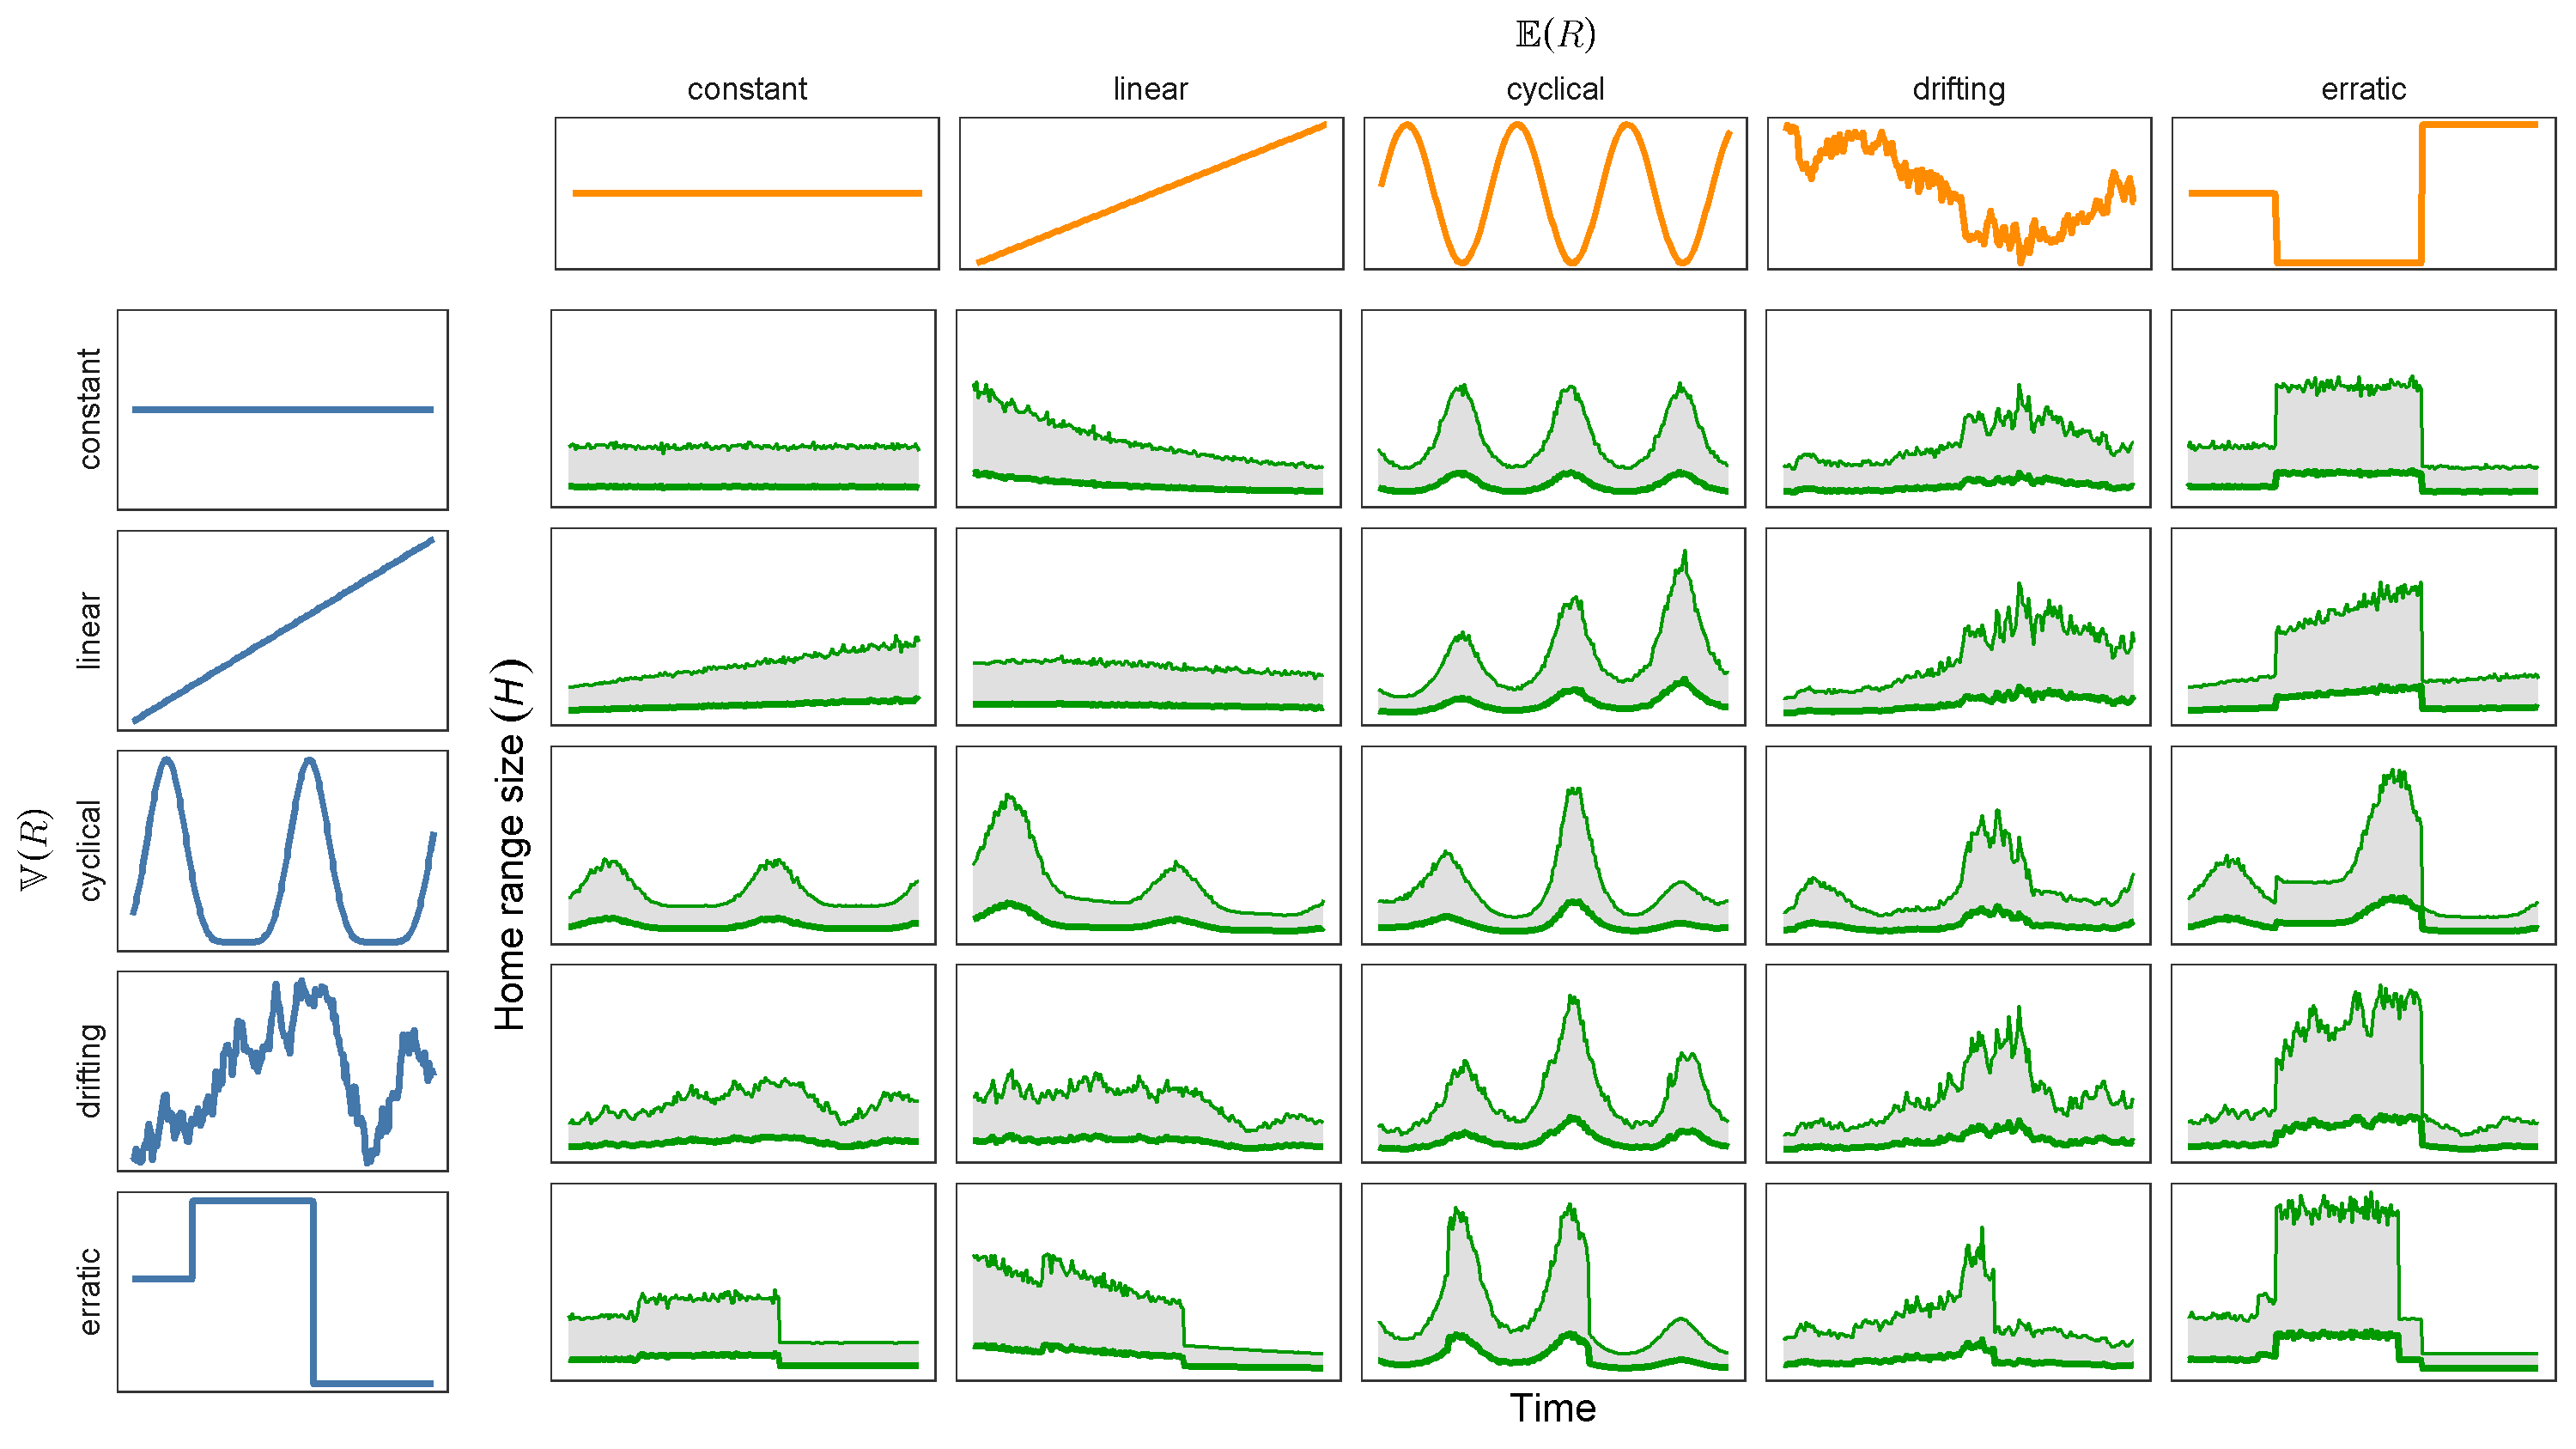
\includegraphics[width=1\linewidth]{../figures/mean-variance-5-by-5-hr-sims} 

}

\caption{Simulated home-range sizes, $H$, of an organism living in habitats where the mean and variance in resources are constant, linearly increasing, cyclical, drifting, or erratic over time (but homogeneous over space for a given $t$). Note how $H$ decreases nonlinearly as $\mu(t)$ increases and increases nonlinearly as $\sigma^2(t)$ increases. Additionally, the variance in $H$ is higher when $\mu(t)$ is lower or $\sigma^2(t)$ is higher, and changes in $\sigma^2(t)$ have greater impacts when $\mu(t)$ is low.}\label{fig:5-5-sims}
\end{figure}

The leftmost column of fig.~\ref{fig:5-5-sims} (constant \(\text{E}(R)\)) illustrates the effects of \(\text{Var}(R)\) on \(H\) while \(\text{E}(R)\) remains constant. Overall, both mean \(H\) and the variance around it increase with \(\sigma^2(t)\) (most visible with constant \(\text{E}(R)\) and linear \(\text{Var}(R)\)). Similarly to resource-poor periods, times of greater stochasticity require the organism to move over larger areas for longer periods of time. Additionally, the greater in uncertainty in how much time and space the organism will require to reach satiety, or indeed whether an organism living in highly stochastic environments can even reach satiety within a finite amount of time.

The remaining panels in fig.~\ref{fig:5-5-sims} illustrate how \(\text{E}(R)\) and \(\text{Var}(R)\) jointly affect \(H\) and how unintuitive the effects can be. Since \(\text{E}(R)\) and \(\text{Var}(R)\) have opposite effects on \(H\), disentangling the effects can be particularly difficult when both parameters change in a correlated manner (e.g., linear \(\text{E}(R)\) and \(\text{Var}(R)\)). When both \(\text{E}(R)\) and \(\text{Var}(R)\) increase linearly, \(H\) initially increases since the effect of \(\text{Var}(R)\) is stronger, but then decreases as the effect of \(\text{E}(R)\) begins to dominate. Difficulties in disentangling the two effects are explored in greater depth in the case study in the following section.

Although the temporal trends in fig.~\ref{fig:5-5-sims} are complex and the effects of \(\text{E}(R)\) and \(\text{Var}(R)\) can be hard to disentangle, two simple relationships emerge when \(H\) is shown as a function of either \(\text{E}(R)\) or \(\text{Var}(R)\), rather than time: \(H\) decreases nonlinearly with \(\text{E}(R)\) and increases with \(\text{Var}(R)\) (panels A and B of fig.~\ref{fig:5-5-reg}). The estimated relationships thus follow the hypothesis we presented in fig.~\ref{fig:hr-hyp}, although we found that the effect of \(\text{Var}(R)\) at average \(\text{E}(R)\) was linear with a slight sublinear saturation at high values of \(\text{Var}(R)\). However, notice that the effect of \(\text{Var}(R)\) on \(E(H)\) depends strongly on \(\text{E}(R)\) (panel C): When \(\text{E}(R)\) is low, \(\text{E}(H)\) is high and \(\text{Var}(R)\) does not have a strong effect, but when \(\text{E}(R)\) is high the effect of \(\text{Var}(R)\) on \(\text{E}(H)\) is exponential. Similarly, \(\text{E}(H)\) decreases exponentially with \(\text{E}(R)\) except when \(\text{Var}(R)\) is very high.

As expected by the changes in the spread of the points in panels A and B of fig.~\ref{fig:5-5-reg}, the variance in \(H\), \(\text{Var}(H)\), also depends on \(\text{E}(R)\) and \(\text{Var}(R)\) (fig.~\ref{fig:5-5-reg}D-F). Since we modeled \(H\) using a Gamma family of distributions, we expected \(\text{Var}(H)\) to increase with \(\text{E}(H)\), but the location-scale model removes the assumption of a constant mean-variance relationship (i.e., constant coefficient of variation, \(\frac{\mu(t)}{\sigma^2(t)}\). This allowed us to show that the effect of \(R\) on \(\text{Var}(H)\) is much stronger than the effect of \(R\) on \(\text{E}(H)\). Consequences of these effects are explored in the discussion section.

\begin{figure}

{\centering 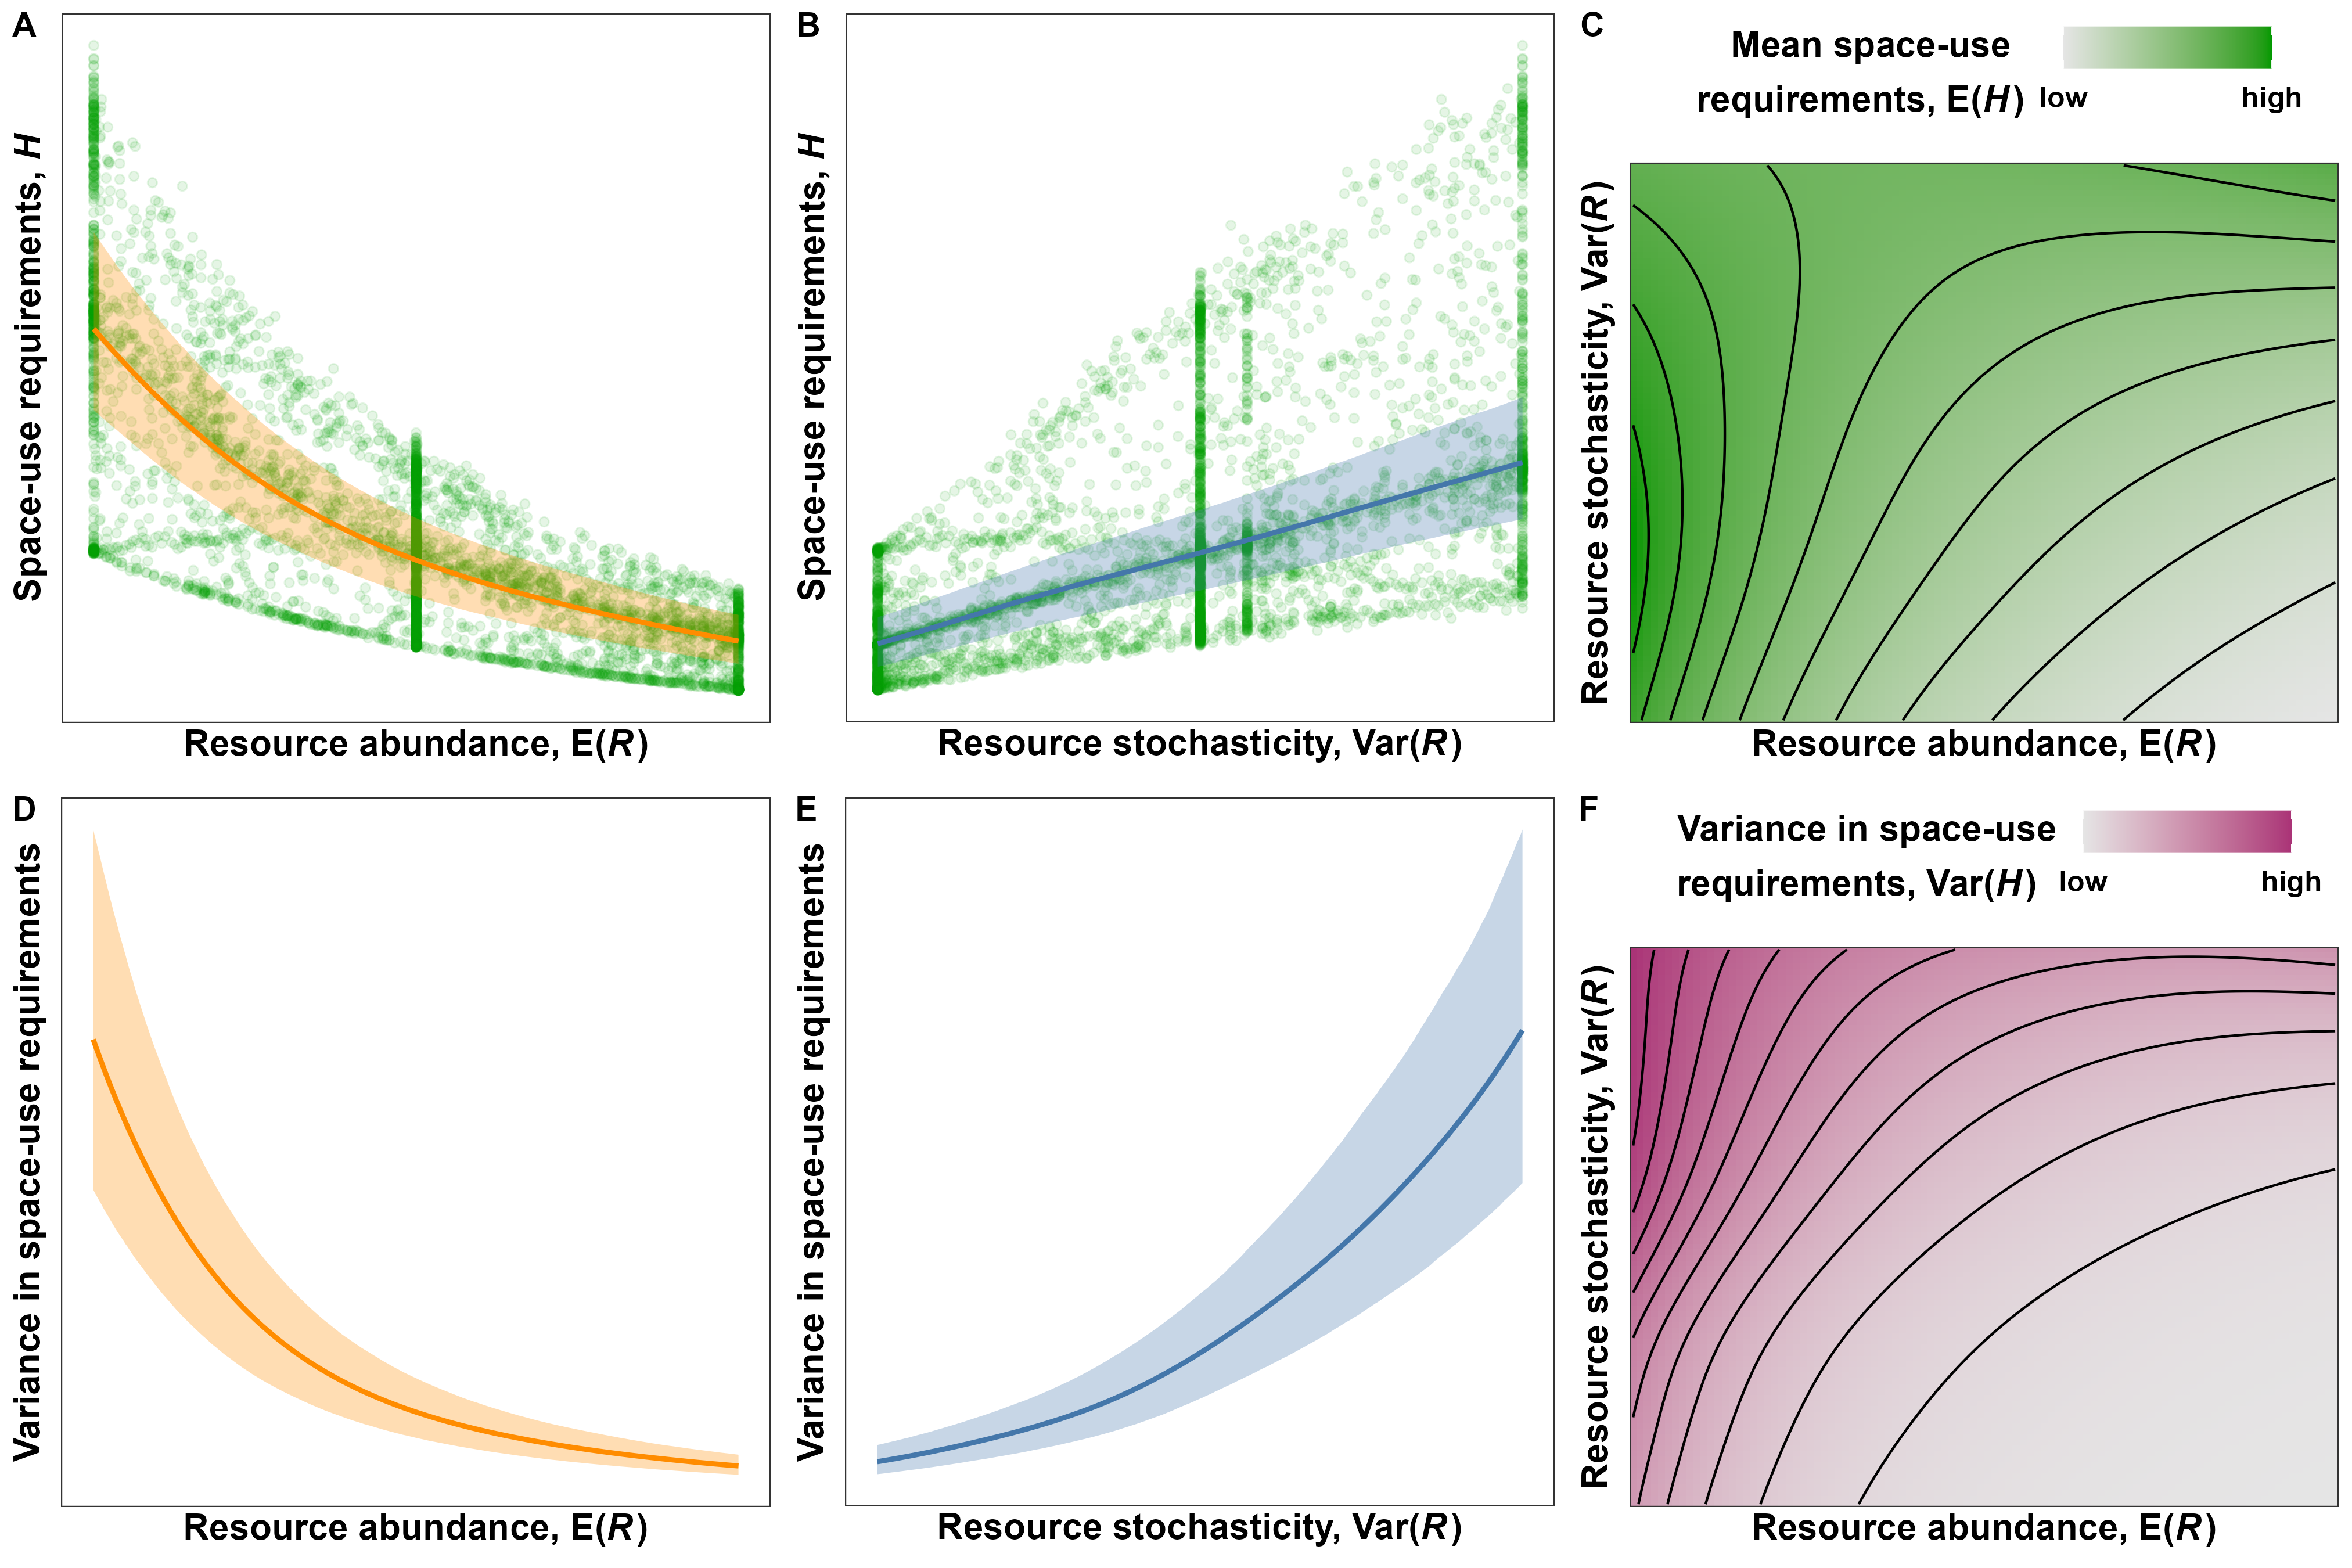
\includegraphics[width=1\linewidth]{../figures/simulation-regression-mean-and-var} 

}

\caption{Effects of $\text{E}(R)$ and $\text{Var}(R)$ on on the mean (A-C) and variance (D-F) in simulated home-range size with 95\% Bayesian credible intervals. While the estimated marginal effect of $\text{Var}(R)$ on $\text{E}(H)$ is sublinear (panel B), the effect of $\text{Var}(R)$ is superlinear for high values of $\text{E}(R)$ (panel C). The relationships were estimated using a Generalized Additive Model for Location and Scale with a Gamma location-scale family of distributions ($\tt{mgcv\!::\!gammals}$). Credible intervals were calculated using 10,000 samples from the posterior distribution while assuming multivariate Gaussian coefficients. Additional details on the model structure are provided in Appendix B.}\label{fig:5-5-reg}
\end{figure}

\section{A case study on a lowland tapir in the Brazilian Cerrado}\label{a-case-study-on-a-lowland-tapir-in-the-brazilian-cerrado}

\noindent The simulations in the section above support the hypothesis we presented in the background section, but they are based on assumptions that are often not met in real natural environments. Organisms live in spatiotemporally heterogeneous and dynamic environments that promote the use of perceptual ranges, navigation, and memory. Together, these abilities result in selective space use that depends on resource availability {[}14{]} and resource depletion {[}15{]}.

In this section, we test the hypothesis using empirical tracking data on a lowland tapir from the Brazilian Cerrado along with empirical estimates of \(\text{E}(R)\) and \(\text{Var}(R)\). We measure \(R\) using Normalized Difference Vegetation Index {[}NDVI, see 76{]}, a remote-sensed measure of landscape greenness, as a proxy for forage abundance. Appendix C contains additional information on how we modeled NDVI and the tapir's movement using continuous-time movement models {[}71,77{]} and autocorrelated kernel density estimation {[}78--80{]}.

Fig. \ref{fig:tapir-mw} illustrates how a tapir in the Brazilian Cerrado adapted its 7-day home-range size to spatiotemporal changes in estimated \(\mu(t, \vec u)\) and \(\sigma^2(t, \vec u)\) (telemetry data from the individual labelled as ``Anna'' in the dataset from {[}29{]}). Panels A and B show the changes in seven-day average mean and variance in NDVI, respectively, experienced by the tapir during the tracking period. The mean and variance in NDVI were estimated using a Generalized Additive Model for Location and Scale {[}GAMLS, 81{]} with a Beta family of distributions (NDVI values ranged from 0.3534 to 0.9475). Panel C shows the changes in the tapir's 7-day home range over time. All 457 of the 7-day windows had a minimum effective sample size of 7 range crossings {[}range: 7.7 -- 69.6, see 82{]}, and 92\% had resolvable (i.e., non-NA) home range crossing times, all of which were below 17 hours. Note how the tapir uses more space during periods of lower NDVI (e.g., August 2017) and less space during periods with high NDVI (January 2018). Additionally, when resources are scarce and highly unpredictable (August 2018), the tapir uses up to 5 times more space than when resources are abundant and predictable (e.g., January 2018). Finally, panels D and E show the estimated (marginal) effects of \(\hat\mu(t, \vec u)\) and \(\hat\sigma^2(t, \vec u)\) on the tapir's 7-day home-range size. Since \(\hat\mu(t, \vec u)\) and \(\hat\sigma^2(t, \vec u)\) are correlated (panel F) and spatiotemporally autocorrelated (panels A, B, and F), the effects of \(R\) on \(H\) should be modeled carefully. To avoid over-fitting the model, we constrained the smooth effects of \(\hat\mu(t, \vec u)\) and \(\hat\sigma^2(t, \vec u)\) and their interaction effect to a small basis size (\(\tt{k = 3}\)). Additional information is provided in appendix C. The results presented in panels D-F of fig.~\ref{fig:tapir-mw} match our findings from the simulations (fig.~\ref{fig:5-5-reg}A-C): The tapir's 7-day home range decreases with \(\hat\mu(t, \vec u)\) and increases with \(\hat\sigma^2(t, \vec u)\), and the effect of \(\hat\mu(t, \vec u)\) depends on \(\hat\sigma^2(t, \vec u)\), and vice-versa. Alone, \(\hat\mu(t, \vec u)\) and \(\hat\sigma^2(t, \vec u)\) cause the tapir to double her home range (panels D and E), but together they result in an approximate 15-fold change in home-range size (observed range: 0.8 to 12.4 km\textsuperscript{2}; see panel F). Additionally, note how high NDVI values (\(\hat \mu(t, \vec u) > 0.8\)) cause \(\hat\sigma^2(t, \vec u)\) to have little to no effect on home-range size, as indicated by the vertical contour line in panel F. Similar conclusions can be drawn for the animal's diffusion (i.e., area covered per unit time), which is a more appropriate measure of space use when animals are not range resident {[}82{]}.

\begin{figure}

{\centering \includegraphics[width=1\linewidth]{../figures/tapir-example} 

}

\caption{Effects of estimated $\mu(t, \vec u)$ and $\sigma^2(t, \vec u)$ on the home-range size of a lowland tapir (\emph{Tapirus terrestris}). (A) Trends in resource abundance over time, $\hat\mu(t, \vec u)$, estimated as the average mean NDVI at the locations visited by the tapir during a seven-day period. (B) Variance in resources over time, $\hat\sigma^2(t, \vec u)$, estimated as the average variance in NDVI at the locations visited by the tapir during a seven-day period. (C) Seven-day 95\% home range estimated using Autocorrelated Kernel Density Estimation. (D, E) Estimated marginal effects of $\hat\mu(t, \vec u)$ and $\hat\sigma^2(t, \vec u)$ on home-range size. The model accounted for the marginal effects of $\hat\mu(t, \vec u)$, $\hat\sigma^2(t, \vec u)$, and their interaction effect. (F) Estimated home-range size in response to changes in both $\hat\mu(t, \vec u)$ and $\hat\sigma^2(t, \vec u)$. Note how the effect of $\hat\sigma^2(t, \vec u)$ is more pronounced when $\hat\mu(t, \vec u)$ is low. See Appendix C for additional information. The tapir movement data corresponds to the individual named ``Anna" from the Cerrado sample of Medici \emph{et al.} [29].}\label{fig:tapir-mw}
\end{figure}

Quantifying the direct effects of \(\text{E}(R)\) and \(\text{Var}(R)\) on \(H\) using empirical data is more complex than with simulated data, and it requires a different causal framework, particularly in the case of observational studies (as opposed to experimentally-controlled studies; see fig.~\ref{fig:dag-empirical}). Unlike with the simulations, \(\text{E}(R)\) and \(\text{Var}(R)\) are not controlled variables and instead depend on the distribution of \(R\), which depends on a variety of other factors (that we exclude from the figure for simplicity). Both \(\text{E}(R)\) and \(\text{Var}(R)\) then impact \(H\) as well as habitat-level variables (e.g., competition, predation, etc.; indicated as \(Z\)) that also affect \(H\). Additionally, estimating \(R\) via a proxy (NDVI) adds satellite-level noise and confounds {[}e.g., saturation, cloud cover, spatiotemporal averaging -- indicated as \(S\), see 83,84,85{]}. However, \(\text{E}(R)\) and \(\text{Var}(R)\) can be correlated to \(\text{E}(\text{NDVI})\) and \(\text{Var}(\text{NDVI})\), respectively, provided that analysts use models that are sufficiently smooth and flexible at the relevant spatiotemporal scale {[}86{]}. We discuss this in further detail in the section below on the strengths and limitations of the empirical approach.

\begin{figure}

{\centering \includegraphics[width=0.75\linewidth]{manuscript_files/figure-latex/dag-empirical-1} 

}

\caption{Directed Acyclical Graph assumed for inferring the causal effects of $\text{E}(R)$ and $\text{Var}(R)$ on $H$, where NDVI was used as a proxy for $R$. $Z$ and $S$ indicate confounds that result from habitat-level variables (e.g., competition, predation, etc.) and satellite-level variables (e.g., noise, cloud cover).}\label{fig:dag-empirical}
\end{figure}

\section{Discussion}\label{discussion}

\noindent The amount of space organisms use is determined by a multitude of factors {[}16{]}, but the search for resources is often a main driver of how much and where organisms move. This paper builds on earlier theoretical work {[}13,e.g., 18,19{]} and presents a unifying hypothesis that describes the effects of resource abundance and stochasticity on organisms' range sizes. We use quantitative simulations and an empirical case study to support the hypothesis and show that it provides a simple framework for understanding how motile organisms adapt their movement in dynamic environments. Separately, resource abundance and stochasticity have simple but opposing effects on organisms' range sizes: \(H\) decreases with \(\text{E}(R)\) and increases with \(\text{Var}(R)\). Together, the degree to which \(\text{E}(R)\) affects \(H\) depends on \(\text{Var}(R)\), and vice-versa, so organisms' responses to resource dynamics can be complex. The simulated and empirical results suggest qualitatively similar marginal effects of \(\text{E}(R)\) and \(\text{Var}(R)\), but there are differences in the estimated interactive effects. In the simulated data, \(\text{Var}(R)\) has little effect when \(\text{E}(R)\) is low and a strong effect when \(\text{E}(R)\) is high, while the opposite is true for the empirical data. This difference is due to two reasons. Firstly, the shape and symmetry of bounded distributions such as Gamma (\(R > 0\)) and Beta (\(0 < R < 1\)) distributions depend on both \(\text{E}(R)\) and \(\text{Var}(R)\) (figs. A3, A4), but \(\text{Var}(R)\) does not affect the shape of a Gamma distribution as much if \(\text{E}(R)\) is low (fig.~B3). Secondly, and perhaps more interestingly, the simulation approach does not account for real-world adaptations to \(\text{E}(R)\) and \(\text{Var}(R)\) such as selective space use, which are included (but not explicitly accounted for) in the empirical approach. Below we discuss the strengths and limitations of each approach.

\subsection{Strengths and limitations of the simulation-based approach}\label{strengths-and-limitations-of-the-simulation-based-approach}

\noindent Our simulations are based on a simplistic environment with many assumptions that allowed us to estimate how resource abundance and stochasticity affect organisms' home-range sizes if organisms can only respond to changes by adapting the amount of time spent searching for food (with no energetic cost to movement). The use of continuous-time movement models coupled with few drivers of movement supported realistic data that could be explained by straightforward causal models. The absence of confounding variables (e.g., predator avoidance, territoriality, competition, landscape connectivity; see fig.~\ref{fig:dag-sims}) or sample size limitation allowed us to ensure estimates were accurate and robust (sensitivity analysis available in Appendix B).

Deviations from the simulations offer a means of detecting when the underlying assumptions are inappropriate and how additional factors may affect organisms' responses to changes in \(\text{E}(R)\) and \(\text{Var}(R)\). For example, energetic costs of movement are often non-negligible and depend on organism size {[}40{]}, movement speed {[}40{]}, and ambient temperature {[}1,87{]}. In addition, an organism may alter its movement behavior, physiology, and energetic needs to buffer itself against changes in \(\text{E}(R)\) and \(\text{Var}(R)\) by using space selectively {[}68,88--90{]} and adapting their behavior and physiology over time {[}18,69{]}. Before or during periods of scarcity, organisms may cache resources {[}91{]}, build up fat reserves {[}45{]}, enter states of dormancy {[}92--94{]}, or even pause fetal growth {[}7{]}. However, organisms may be unable to respond to changes in \(\text{E}(R)\) and \(\text{Var}(R)\) optimally due to various reasons, including limited perceptive range {[}61{]}, lack of experience {[}9,47,63--65,95{]}, avoidance of competitors and predators {[}14,96{]}, or a physiology that is not amenable to things like hibernation or fat storage. Thus, organisms may relocate their range to a sub-optimal location {[}33,34,97,98{]}, which may exacerbate the effects of \(\text{E}(R)\) and \(\text{Var}(R)\) on both mean range size and the variance around it.

\subsection{Strengths and limitations of the empirical approach}\label{strengths-and-limitations-of-the-empirical-approach}

\noindent There are two main advantages of taking an empirical approach. Firstly, modeling real-world animal movement data can produce scale-appropriate and easily interpretable estimates. Secondly, empirical data contain information on the effects of \(\text{E}(R)\), \(\text{Var}(R)\), and confounding variables without having to design complex and time-consuming simulations. However, it is not always possible to quantify confounding variables. For example, while there may be some appropriate proxies of competition, such as density of competitors, these variables may be hard to quantify, and they may not account for the confounding effects appropriately (i.e., the presence of competitors may not reflect competitive pressure). This is problematic if one is interested in estimating the direct causal effect of \(\text{E}(R)\) and \(\text{Var}(R)\), which requires removing any non-negligible confounding effects {[}75{]}.

Similarly, if \(R\) non-measurable (as is often the case), \(R\) must be estimated with proxies such as NDVI {[}76{]}, which may introduce complexities. While \(R\) and NDVI are correlated for many species {[}e.g., 45,46,95,99--101{]}, the relationship between the two can be weak {[}84{]}, satellite-dependent {[}85{]}, and nonlinear {[}83,85{]}. This complexity can introduce two sources of bias: ecosystem-level biases (indicated as \(Z\) in the directed acyclical graph in fig.~\ref{fig:dag-empirical}) and satellite-level confounding variables (\(S\) in fig.~\ref{fig:dag-empirical}). Examples of ecosystem-level biases are the effects of competition, predation, habitat connectivity, and movement costs, all of which can depend on habitat quality, and, consequently, be correlated nonlinearly to \(R\) and NDVI {[}35,102{]}. Resource-rich patches can attract larger amounts of competitors {[}14{]} and predators {[}20{]}, which may, in turn, increase pressures from competition and predation {[}15,39{]}. However, such pressures may result in both an expansion of the range {[}35,102{]} or a contraction, since larger ranges can be harder to defend and result in higher movement costs {[}35,103{]} and encounter rates {[}104{]}. Satellite-level confounds include information loss due to coarse spatiotemporal resolution {[}83,85{]}, satellite-level error {[}83,85,105{]}, and other limitations of remote sensing (e.g., inability to quantify specific resources or small-scale resource depletion). However, nonlinear models such as Generalized Additive Models {[}106{]} can help account for preferences for intermediate values of remotely-sensed \(R\) {[}e.g., young grass rather than mature grasslands, see 85{]}.

\section{Conclusions}\label{conclusions}

\noindent The work presented here provides a unifying framework for viewing movement as a response to resource abundance and stochasticity. We provide a sensible and unifying hypothesis of the effects of \(\text{E}(R)\) and \(\text{Var}(R)\) on organisms' range sizes and movement behavior. We demonstrate that organisms' range sizes decrease with resource abundance, increase with resource stochasticity, and that the effects of \(\text{Var}(R)\) can depend strongly on \(\text{E}(R)\).

Recent advances in computational power have greatly increased analysts' ability to fit computationally demanding models {[}107,108{]} that allow biologists to move beyond only considering changes in mean conditions. By accounting for changes in stochasticity, we can start developing a more comprehensive understanding of how organisms adapt to the dynamic environments organisms live in, including recent changes in climate {[}109{]} and increases in the frequency and intensity of extreme events {[}66,67,110--112{]}.

\section{List of abbreviations}\label{list-of-abbreviations}

\begin{tabular}{l|l}
\hline
\textbf{Abbreviation} & \textbf{Definition}\\
\hline
$H$ & Range size\\
\hline
$\hat H_{95\%}$ & Estimated $95\%$ home range size\\
\hline
$C$ & Resource consumption rate\\
\hline
$R$ & Resources\\
\hline
$t$ & Moment in time\\
\hline
$\vec u$ & Location in space (vector of coordinates)\\
\hline
$\text{E}(R)$ & Resource abundance\\
\hline
$\mu(t)$ & Resource abundance as a function of time\\
\hline
$\mu(t, \vec u)$ & Resource abundance as a function of time and space\\
\hline
$\text{Var}(R)$ & Resource stochasticity\\
\hline
$\sigma^2(t)$ & Resource stochasticity as a function of time\\
\hline
$\sigma^2(t, \vec u)$ & Resource stochasticity as a function of time and space\\
\hline
$\hat{\varsigma^2}$ & Estimated positional variance\\
\hline
$\Gamma(\mu, \sigma^2)$ & Gamma distribution with mean $\mu$ and variance $\sigma^2$\\
\hline
NDVI & Normalized Difference Vegetation Index\\
\hline
GAMLS & Generalized Additive Model for Location and Scale\\
\hline
\end{tabular}

\section{Declarations}\label{declarations}

\subsection{Ethics approval and consent to participate}\label{ethics-approval-and-consent-to-participate}

\noindent Not applicable.

\subsection{Consent for publication}\label{consent-for-publication}

\noindent Not applicable.

\subsection{Availability of data and materials}\label{availability-of-data-and-materials}

\noindent All code and data used for this manuscript is available on GitHub at \url{https://github.com/QuantitativeEcologyLab/hr-resource-stoch}, with the exception of two simulated datasets that were greater than 100 MB and the tapir data. The simulated data can be produced by running the scripts in the repository, while the tapir data is available at \url{https://github.com/StefanoMezzini/tapirs}.

\subsection{Competing interests}\label{competing-interests}

\noindent The authors declare that they have no competing interests.

\subsection{Funding}\label{funding}

\noindent SM was supported by funding from the University of British Columbia Okanagan, the Canadian Foundation for Innovation, BC Parks Living Labs, and MITACS. MJN was supported by NSERC Discovery Grant RGPIN-2021-02758 and the Canadian Foundation for Innovation. CHF was supported by NSF IIBR 1915347.

\subsection{Authors' contributions}\label{authors-contributions}

\noindent SM performed the literature review, designed the simulations, analyzed the data, and wrote the manuscript. CHF contributed to the analyses. EPM provided the tapir telemetry data. MJN conceived the project idea and provided support throughout the analyses. All authors contributed to the writing and read and approved the final manuscript.

\subsection{Acknowledgements}\label{acknowledgements}

\noindent We would like to thank Dr.~Simon Wood for providing code to fit a Beta location-scale GAM despite not being involved directly with the project. Additionally, we thank all those who provided feedback on all posters, presentation, and writings related to this project. In particular, we thank all those who provided feedback on the manuscript and appendices despite not being authors, namely, in alphabetical order by first name: Aimee Chhen, Jessa Marley, Kim Hinz, Lauren Mills, Sarah Wyse, and Dr.~Simon Wood.

\subsection{Authors' information}\label{authors-information}

\noindent See page 1 for affiliations.

\noindent Authors' emails:

\noindent SM: \(\text{stefano.mezzini@ubc.ca}\)

\noindent CHF: \(\text{christen.fleming@ucf.edu}\)

\noindent EPM: \(\text{medici@ipe.org.br}\)

\noindent MJN: \(\text{michael.noonan@ubc.ca}\)

\clearpage

\newpage

\section{References}\label{references}

\hangparas{1em}{1}

\phantomsection\label{refs}
\begin{CSLReferences}{0}{1}
\bibitem[\citeproctext]{ref-hou_cold_2020}
1. Hou R, Chapman CA, Jay O, Guo S, Li B, Raubenheimer D. Cold and hungry: Combined effects of low temperature and resource scarcity on an edge‐of‐range temperate primate, the golden snub‐nose monkey. Ecography {[}Internet{]}. 2020 {[}cited 2022 Oct 3{]};43:1672--82. Available from: \url{https://onlinelibrary.wiley.com/doi/10.1111/ecog.05295}

\bibitem[\citeproctext]{ref-le_bot_fishery_2019}
2. Le Bot T, Lescroël A, Fort J, Péron C, Gimenez O, Provost P, et al. Fishery discards do not compensate natural prey shortage in northern gannets from the english channel. Biological Conservation {[}Internet{]}. 2019 {[}cited 2022 Oct 3{]};236:375--84. Available from: \url{https://linkinghub.elsevier.com/retrieve/pii/S0006320718310930}

\bibitem[\citeproctext]{ref-dai_pra_ground_2022}
3. Dai Pra R, Mohr SM, Merriman DK, Bagriantsev SN, Gracheva EO. Ground squirrels initiate sexual maturation during hibernation. Current Biology {[}Internet{]}. 2022 {[}cited 2022 Sep 2{]};32:1822--1828.e4. Available from: \url{https://linkinghub.elsevier.com/retrieve/pii/S0960982222002548}

\bibitem[\citeproctext]{ref-rocha_life_2021}
4. Rocha JL, Godinho R, Brito JC, Nielsen R. Life in deserts: The genetic basis of mammalian desert adaptation. Trends in Ecology \& Evolution {[}Internet{]}. 2021 {[}cited 2022 Sep 2{]};36:637--50. Available from: \url{https://linkinghub.elsevier.com/retrieve/pii/S0169534721000744}

\bibitem[\citeproctext]{ref-wessling_seasonal_2018}
5. Wessling EG, Deschner T, Mundry R, Pruetz JD, Wittig RM, Kühl HS. Seasonal variation in physiology challenges the notion of chimpanzees (pan troglodytes verus) as a forest-adapted species. Front Ecol Evol {[}Internet{]}. 2018 {[}cited 2022 Sep 2{]};6:60. Available from: \url{http://journal.frontiersin.org/article/10.3389/fevo.2018.00060/full}

\bibitem[\citeproctext]{ref-stefanescu_timing_2021}
6. Stefanescu C, Ubach A, Wiklund C. Timing of mating, reproductive status and resource availability in relation to migration in the painted lady butterfly. Animal Behaviour {[}Internet{]}. 2021 {[}cited 2022 Sep 2{]};172:145--53. Available from: \url{https://linkinghub.elsevier.com/retrieve/pii/S0003347220303742}

\bibitem[\citeproctext]{ref-schmidt_interplay_2020}
7. Schmidt NM, Grøndahl C, Evans AL, Desforges J-P, Blake J, Hansen LH, et al. On the interplay between hypothermia and reproduction in a high arctic ungulate. Sci Rep {[}Internet{]}. 2020 {[}cited 2022 Sep 2{]};10:1514. Available from: \url{http://www.nature.com/articles/s41598-020-58298-8}

\bibitem[\citeproctext]{ref-douglas_relative_2014}
8. Douglas DJT, Pearce-Higgins JW. Relative importance of prey abundance and habitat structure as drivers of shorebird breeding success and abundance: Drivers of shorebird breeding success and abundance. Anim Conserv {[}Internet{]}. 2014 {[}cited 2022 Nov 8{]};17:535--43. Available from: \url{https://onlinelibrary.wiley.com/doi/10.1111/acv.12119}

\bibitem[\citeproctext]{ref-foley_severe_2008}
9. Foley C, Pettorelli N, Foley L. Severe drought and calf survival in elephants. Biology Letters {[}Internet{]}. 2008 {[}cited 2020 Feb 12{]};4:541--4. Available from: \url{https://royalsocietypublishing.org/doi/10.1098/rsbl.2008.0370}

\bibitem[\citeproctext]{ref-berger_climate_2018}
10. Berger J, Hartway C, Gruzdev A, Johnson M. Climate degradation and extreme icing events constrain life in cold-adapted mammals. Scientific Reports {[}Internet{]}. 2018 {[}cited 2020 Jan 24{]};8:1156. Available from: \url{http://www.nature.com/articles/s41598-018-19416-9}

\bibitem[\citeproctext]{ref-van_haastert_food_2009}
11. Van Haastert PJM, Bosgraaf L. Food searching strategy of amoeboid cells by starvation induced run length extension. Dornhaus A, editor. {PLoS} {ONE} {[}Internet{]}. 2009 {[}cited 2025 Feb 6{]};4:e6814. Available from: \url{https://dx.plos.org/10.1371/journal.pone.0006814}

\bibitem[\citeproctext]{ref-taub_root_1996}
12. Taub DR, Goldberg D. Root system topology of plants from habitats differing in soil resource availability. Functional Ecology {[}Internet{]}. 1996 {[}cited 2025 Feb 6{]};10:258. Available from: \url{https://www.jstor.org/stable/2389851?origin=crossref}

\bibitem[\citeproctext]{ref-harestad_home_1979}
13. Harestad AS, Bunnel FL. Home range and body weight--a reevaluation. Ecology {[}Internet{]}. 1979 {[}cited 2022 Sep 5{]};60:389--402. Available from: \url{http://doi.wiley.com/10.2307/1937667}

\bibitem[\citeproctext]{ref-kacelnik_ideal_1992}
14. Kacelnik A, Krebs JR, Bernstein C. The ideal free distribution and predator-prey populations. Trends in Ecology \& Evolution {[}Internet{]}. 1992 {[}cited 2024 Jan 31{]};7:50--5. Available from: \url{https://linkinghub.elsevier.com/retrieve/pii/016953479290106L}

\bibitem[\citeproctext]{ref-charnov_optimal_1976}
15. Charnov EL. Optimal foraging, the marginal value theorem. Theoretical Population Biology {[}Internet{]}. 1976 {[}cited 2024 Jan 31{]};9:129--36. Available from: \url{https://linkinghub.elsevier.com/retrieve/pii/004058097690040X}

\bibitem[\citeproctext]{ref-nathan_movement_2008}
16. Nathan R, Getz WM, Revilla E, Holyoak M, Kadmon R, Saltz D, et al. A movement ecology paradigm for unifying organismal movement research. Proc Natl Acad Sci USA {[}Internet{]}. 2008 {[}cited 2022 Mar 9{]};105:19052--9. Available from: \url{https://pnas.org/doi/full/10.1073/pnas.0800375105}

\bibitem[\citeproctext]{ref-burt_territoriality_1943}
17. Burt WH. Territoriality and home range concepts as applied to mammals. Journal of Mammalogy {[}Internet{]}. 1943 {[}cited 2022 Jan 31{]};24:346. Available from: \url{https://academic.oup.com/jmammal/article-lookup/doi/10.2307/1374834}

\bibitem[\citeproctext]{ref-southwood_habitat_1977}
18. Southwood TRE. Habitat, the templet for ecological strategies? The Journal of Animal Ecology {[}Internet{]}. 1977 {[}cited 2022 Feb 4{]};46:336. Available from: \url{https://www.jstor.org/stable/3817?origin=crossref}

\bibitem[\citeproctext]{ref-stephens_optimal_1982}
19. Stephens DW, Charnov EL. Optimal foraging: Some simple stochastic models. Behav Ecol Sociobiol {[}Internet{]}. 1982 {[}cited 2024 Jan 31{]};10:251--63. Available from: \url{http://link.springer.com/10.1007/BF00302814}

\bibitem[\citeproctext]{ref-duncan_lifehistory_2015}
20. Duncan C, Nilsen EB, Linnell JDC, Pettorelli N. Life‐history attributes and resource dynamics determine intraspecific home‐range sizes in carnivora. Remote Sens Ecol Conserv {[}Internet{]}. 2015 {[}cited 2024 May 29{]};1:39--50. Available from: \url{https://zslpublications.onlinelibrary.wiley.com/doi/10.1002/rse2.6}

\bibitem[\citeproctext]{ref-rizzuto_forage_2021}
21. Rizzuto M, Leroux SJ, Vander Wal E, Richmond IC, Heckford TR, Balluffi-Fry J, et al. Forage stoichiometry predicts the home range size of a small terrestrial herbivore. Oecologia {[}Internet{]}. 2021 {[}cited 2022 Mar 2{]};197:327--38. Available from: \url{https://link.springer.com/10.1007/s00442-021-04965-0}

\bibitem[\citeproctext]{ref-broekman_environmental_2024}
22. Broekman MJE, Hilbers JP, Hoeks S, Huijbregts MAJ, Schipper AM, Tucker MA. Environmental drivers of global variation in home range size of terrestrial and marine mammals. Journal of Animal Ecology {[}Internet{]}. 2024 {[}cited 2024 Jul 29{]};93:488--500. Available from: \url{https://besjournals.onlinelibrary.wiley.com/doi/10.1111/1365-2656.14073}

\bibitem[\citeproctext]{ref-singh_migration_2012}
23. Singh NJ, Börger L, Dettki H, Bunnefeld N, Ericsson G. From migration to nomadism: Movement variability in a northern ungulate across its latitudinal range. Ecological Applications {[}Internet{]}. 2012 {[}cited 2022 Nov 17{]};22:2007--20. Available from: \url{http://doi.wiley.com/10.1890/12-0245.1}

\bibitem[\citeproctext]{ref-wheat_migrate_2017}
24. Wheat RE, Lewis SB, Wang Y, Levi T, Wilmers CC. To migrate, stay put, or wander? Varied movement strategies in bald eagles (haliaeetus leucocephalus). Mov Ecol {[}Internet{]}. 2017 {[}cited 2022 Oct 17{]};5:9. Available from: \url{http://movementecologyjournal.biomedcentral.com/articles/10.1186/s40462-017-0102-4}

\bibitem[\citeproctext]{ref-teitelbaum_beyond_2019}
25. Teitelbaum CS, Mueller T. Beyond migration: Causes and consequences of nomadic animal movements. Trends in Ecology \& Evolution {[}Internet{]}. 2019 {[}cited 2022 Feb 1{]};34:569--81. Available from: \url{https://linkinghub.elsevier.com/retrieve/pii/S0169534719300527}

\bibitem[\citeproctext]{ref-chevin_adaptation_2010}
26. Chevin L-M, Lande R, Mace GM. Adaptation, plasticity, and extinction in a changing environment: Towards a predictive theory. Kingsolver JG, editor. {PLoS} Biology {[}Internet{]}. 2010 {[}cited 2020 Nov 11{]};8:e1000357. Available from: \url{https://dx.plos.org/10.1371/journal.pbio.1000357}

\bibitem[\citeproctext]{ref-herfindal_prey_2005}
27. Herfindal I, Linnell JDC, Odden J, Nilsen EB, Andersen R. Prey density, environmental productivity and home‐range size in the eurasian lynx ( \emph{lynx lynx} ). Journal of Zoology {[}Internet{]}. 2005 {[}cited 2022 Sep 23{]};265:63--71. Available from: \url{https://onlinelibrary.wiley.com/doi/10.1017/S0952836904006053}

\bibitem[\citeproctext]{ref-nilsen_can_2005}
28. Nilsen EB, Herfindal I, Linnell JDC. Can intra-specific variation in carnivore home-range size be explained using remote-sensing estimates of environmental productivity? Écoscience {[}Internet{]}. 2005 {[}cited 2021 Nov 29{]};12:68--75. Available from: \url{https://www.tandfonline.com/doi/full/10.2980/i1195-6860-12-1-68.1}

\bibitem[\citeproctext]{ref-medici_movement_2022}
29. Medici EP, Mezzini S, Fleming CH, Calabrese JM, Noonan MJ. Movement ecology of vulnerable lowland tapirs between areas of varying human disturbance. Mov Ecol {[}Internet{]}. 2022 {[}cited 2022 Mar 14{]};10:14. Available from: \url{https://movementecologyjournal.biomedcentral.com/articles/10.1186/s40462-022-00313-w}

\bibitem[\citeproctext]{ref-lindstedt_seasonality_1985}
30. Lindstedt SL, Boyce MS. Seasonality, fasting endurance, and body size in mammals. The American Naturalist {[}Internet{]}. 1985 {[}cited 2022 Feb 4{]};125:873--8. Available from: \url{https://www.journals.uchicago.edu/doi/10.1086/284385}

\bibitem[\citeproctext]{ref-morellet_seasonality_2013}
31. Morellet N, Bonenfant C, Börger L, Ossi F, Cagnacci F, Heurich M, et al. Seasonality, weather and climate affect home range size in roe deer across a wide latitudinal gradient within europe. Coulson T, editor. Journal of Animal Ecology {[}Internet{]}. 2013 {[}cited 2020 Nov 11{]};82:1326--39. Available from: \url{http://doi.wiley.com/10.1111/1365-2656.12105}

\bibitem[\citeproctext]{ref-fjelldal_nightly_2021}
32. Fjelldal MA, Wright J, Stawski C. Nightly torpor use in response to weather conditions and individual state in an insectivorous bat. Oecologia {[}Internet{]}. 2021 {[}cited 2022 Oct 3{]};197:129--42. Available from: \url{https://link.springer.com/10.1007/s00442-021-05022-6}

\bibitem[\citeproctext]{ref-torrez-herrera_monkeys_2020}
33. Tórrez-Herrera LL, Davis GH, Crofoot MC. Do monkeys avoid areas of home range overlap because they are dangerous? A test of the risk hypothesis in white-faced capuchin monkeys (cebus capucinus). Int J Primatol {[}Internet{]}. 2020 {[}cited 2022 Mar 9{]};41:246--64. Available from: \url{http://link.springer.com/10.1007/s10764-019-00110-0}

\bibitem[\citeproctext]{ref-rich_anthropogenic_2012}
34. Rich LN, Mitchell MS, Gude JA, Sime CA. Anthropogenic mortality, intraspecific competition, and prey availability influence territory sizes of wolves in montana. J Mammal {[}Internet{]}. 2012 {[}cited 2022 Mar 10{]};93:722--31. Available from: \url{https://academic.oup.com/jmammal/article-lookup/doi/10.1644/11-MAMM-A-079.2}

\bibitem[\citeproctext]{ref-jetz_scaling_2004}
35. Jetz W, Carbone C, Fulford J, Brown JH. The scaling of animal space use. Science {[}Internet{]}. 2004 {[}cited 2022 Mar 3{]};306:266--8. Available from: \url{https://www.science.org/doi/10.1126/science.1102138}

\bibitem[\citeproctext]{ref-harvey_primate_1981}
36. Harvey PH, Clutton-Brock TH. Primate home-range size and metabolic needs. Behav Ecol Sociobiol {[}Internet{]}. 1981 {[}cited 2022 Nov 12{]};8:151--5. Available from: \url{http://link.springer.com/10.1007/BF00300828}

\bibitem[\citeproctext]{ref-baldwin_nutritional_1984}
37. Baldwin R, Bywater A. \href{https://doi.org/10.1146/annurev.nu.04.070184.000533}{Nutritional energetics of animals}. Annual review of nutrition. 1984;4:101--14.

\bibitem[\citeproctext]{ref-reich_body_2001}
38. Reich PB. Body size, geometry, longevity and metabolism: Do plant leaves behave like animal bodies? Trends in Ecology \& Evolution {[}Internet{]}. 2001 {[}cited 2022 Oct 17{]};16:674--80. Available from: \url{https://linkinghub.elsevier.com/retrieve/pii/S0169534701023060}

\bibitem[\citeproctext]{ref-brown_ecology_1999}
39. Brown JS, Laundre JW, Gurung M. The ecology of fear: Optimal foraging, game theory, and trophic interactions. Journal of Mammalogy {[}Internet{]}. 1999 {[}cited 2024 Jan 31{]};80:385--99. Available from: \url{https://academic.oup.com/jmammal/article-lookup/doi/10.2307/1383287}

\bibitem[\citeproctext]{ref-taylor_energetics_1982}
40. Taylor CR, Heglund NC, Maloiy GM. Energetics and mechanics of terrestrial locomotion. I. Metabolic energy consumption as a function of speed and body size in birds and mammals. Journal of Experimental Biology {[}Internet{]}. 1982 {[}cited 2022 Dec 12{]};97:1--21. Available from: \url{https://journals.biologists.com/jeb/article/97/1/1/34642/Energetics-and-mechanics-of-terrestrial-locomotion}

\bibitem[\citeproctext]{ref-relyea_home_2000}
41. Relyea RA, Lawrence RK, Demarais S. Home range of desert mule deer: Testing the body-size and habitat-productivity hypotheses. The Journal of Wildlife Management {[}Internet{]}. 2000 {[}cited 2021 Nov 29{]};64:146. Available from: \url{https://www.jstor.org/stable/3802984?origin=crossref}

\bibitem[\citeproctext]{ref-dawe_influence_2014}
42. Dawe KL, Bayne EM, Boutin S. Influence of climate and human land use on the distribution of white-tailed deer ( \emph{odocoileus} \emph{virginianus} ) in the western boreal forest. Canadian Journal of Zoology {[}Internet{]}. 2014 {[}cited 2020 Oct 23{]};92:353--63. Available from: \url{http://www.nrcresearchpress.com/doi/10.1139/cjz-2013-0262}

\bibitem[\citeproctext]{ref-berger-tal_invisible_2019}
43. Berger-Tal O, Saltz D. Invisible barriers: Anthropogenic impacts on inter- and intra-specific interactions as drivers of landscape-independent fragmentation. Phil Trans R Soc B {[}Internet{]}. 2019 {[}cited 2022 Aug 11{]};374:20180049. Available from: \url{https://royalsocietypublishing.org/doi/10.1098/rstb.2018.0049}

\bibitem[\citeproctext]{ref-samarra_movements_2017}
44. Samarra FIP, Tavares SB, Béesau J, Deecke VB, Fennell A, Miller PJO, et al. Movements and site fidelity of killer whales (orcinus orca) relative to seasonal and long-term shifts in herring (clupea harengus) distribution. Mar Biol {[}Internet{]}. 2017 {[}cited 2022 Nov 7{]};164:159. Available from: \url{http://link.springer.com/10.1007/s00227-017-3187-9}

\bibitem[\citeproctext]{ref-middleton_green-wave_2018}
45. Middleton AD, Merkle JA, McWhirter DE, Cook JG, Cook RC, White PJ, et al. Green-wave surfing increases fat gain in a migratory ungulate. Oikos {[}Internet{]}. 2018 {[}cited 2022 Sep 2{]};127:1060--8. Available from: \url{https://onlinelibrary.wiley.com/doi/10.1111/oik.05227}

\bibitem[\citeproctext]{ref-geremia_migrating_2019}
46. Geremia C, Merkle JA, Eacker DR, Wallen RL, White PJ, Hebblewhite M, et al. Migrating bison engineer the green wave. Proc Natl Acad Sci {USA} {[}Internet{]}. 2019 {[}cited 2022 Mar 2{]};116:25707--13. Available from: \url{http://www.pnas.org/lookup/doi/10.1073/pnas.1913783116}

\bibitem[\citeproctext]{ref-polansky_elucidating_2015}
47. Polansky L, Kilian W, Wittemyer G. Elucidating the significance of spatial memory on movement decisions by african savannah elephants using state--space models. Proc R Soc B {[}Internet{]}. 2015 {[}cited 2022 Feb 10{]};282:20143042. Available from: \url{https://royalsocietypublishing.org/doi/10.1098/rspb.2014.3042}

\bibitem[\citeproctext]{ref-nandintsetseg_variability_2019}
48. Nandintsetseg D, Bracis C, Leimgruber P, Kaczensky P, Buuveibaatar B, Lkhagvasuren B, et al. Variability in nomadism: Environmental gradients modulate the movement behaviors of dryland ungulates. Ecosphere {[}Internet{]}. 2019 {[}cited 2020 Nov 11{]};10. Available from: \url{https://onlinelibrary.wiley.com/doi/abs/10.1002/ecs2.2924}

\bibitem[\citeproctext]{ref-teitelbaum_how_2015}
49. Teitelbaum CS, Fagan WF, Fleming CH, Dressler G, Calabrese JM, Leimgruber P, et al. How far to go? Determinants of migration distance in land mammals. Festa-Bianchet M, editor. Ecol Lett {[}Internet{]}. 2015 {[}cited 2022 Sep 23{]};18:545--52. Available from: \url{https://onlinelibrary.wiley.com/doi/10.1111/ele.12435}

\bibitem[\citeproctext]{ref-poessel_interpreting_2022}
50. Poessel SA, Woodbridge B, Smith BW, Murphy RK, Bedrosian BE, Bell DA, et al. Interpreting long‐distance movements of non‐migratory golden eagles: Prospecting and nomadism? Ecosphere {[}Internet{]}. 2022 {[}cited 2022 Nov 18{]};13. Available from: \url{https://onlinelibrary.wiley.com/doi/10.1002/ecs2.4072}

\bibitem[\citeproctext]{ref-pretorius_movement_2020}
51. Pretorius MD, Leeuwner L, Tate GJ, Botha A, Michael MD, Durgapersad K, et al. Movement patterns of lesser flamingos \emph{phoeniconaias minor} : Nomadism or partial migration? Wildlife Biology {[}Internet{]}. 2020 {[}cited 2022 Nov 17{]};2020:1--11. Available from: \url{https://onlinelibrary.wiley.com/doi/10.2981/wlb.00728}

\bibitem[\citeproctext]{ref-bista_effect_2022}
52. Bista D, Baxter GS, Hudson NJ, Lama ST, Murray PJ. Effect of disturbances and habitat fragmentation on an arboreal habitat specialist mammal using {GPS} telemetry: A case of the red panda. Landsc Ecol {[}Internet{]}. 2022 {[}cited 2022 Aug 24{]};37:795--809. Available from: \url{https://link.springer.com/10.1007/s10980-021-01357-w}

\bibitem[\citeproctext]{ref-bradsworth_using_2022}
53. Bradsworth N, White JG, Rendall AR, Carter N, Whisson DA, Cooke R. Using thresholds to determine priorities for apex predator conservation in an urban landscape. Landscape and Urban Planning {[}Internet{]}. 2022 {[}cited 2022 Oct 18{]};228:104559. Available from: \url{https://github.com/ropensci/MODIStsp}

\bibitem[\citeproctext]{ref-mcclintic_effects_2014}
54. McClintic LF, Taylor JD, Jones JC, Singleton RD, Wang G. Effects of spatiotemporal resource heterogeneity on home range size of american beaver. J Zool {[}Internet{]}. 2014 {[}cited 2022 Nov 12{]};293:134--41. Available from: \url{https://onlinelibrary.wiley.com/doi/10.1111/jzo.12128}

\bibitem[\citeproctext]{ref-lucherini_habitat_1996}
55. Lucherini M, Lovari S. Habitat richness affects home range size in the red fox vulpes vulpes. Behavioural Processes {[}Internet{]}. 1996 {[}cited 2021 Nov 29{]};36:103--5. Available from: \url{https://linkinghub.elsevier.com/retrieve/pii/0376635795000186}

\bibitem[\citeproctext]{ref-watson_ferruginous_2020}
56. Watson J. Ferruginous hawk (buteo regalis) home range and resource use on northern grasslands in canada. 2020 {[}cited 2022 Nov 8{]}; Available from: \url{http://rgdoi.net/10.13140/RG.2.2.32404.32648}

\bibitem[\citeproctext]{ref-simcharoen_female_2014}
57. Simcharoen A, Savini T, Gale GA, Simcharoen S, Duangchantrasiri S, Pakpien S, et al. Female tiger \emph{panthera tigris} home range size and prey abundance: Important metrics for management. Oryx {[}Internet{]}. 2014 {[}cited 2022 Nov 8{]};48:370--7. Available from: \url{https://www.cambridge.org/core/product/identifier/S0030605312001408/type/journal_article}

\bibitem[\citeproctext]{ref-campillo_effect_2012}
58. Campillo F, Lobry C. Effect of population size in a predator--prey model. Ecological Modelling {[}Internet{]}. 2012 {[}cited 2025 Feb 6{]};246:1--10. Available from: \url{https://linkinghub.elsevier.com/retrieve/pii/S0304380012003432}

\bibitem[\citeproctext]{ref-lee_effects_2011}
59. Lee S-H. Effects of the probability of a predator catching prey on predator--prey system stability. Journal of Asia-Pacific Entomology {[}Internet{]}. 2011 {[}cited 2025 Feb 7{]};14:159--62. Available from: \url{https://linkinghub.elsevier.com/retrieve/pii/S1226861510001329}

\bibitem[\citeproctext]{ref-levin_problem_1992}
60. Levin SA. The problem of pattern and scale in ecology: The robert h. {MacArthur} award lecture. Ecology {[}Internet{]}. 1992 {[}cited 2024 Jan 31{]};73:1943--67. Available from: \url{https://esajournals.onlinelibrary.wiley.com/doi/10.2307/1941447}

\bibitem[\citeproctext]{ref-steixner-kumar_strategies_2020}
61. Steixner-Kumar S, Gläscher J. Strategies for navigating a dynamic world. Science {[}Internet{]}. 2020 {[}cited 2022 Mar 9{]};369:1056--7. Available from: \url{https://www.science.org/doi/10.1126/science.abd7258}

\bibitem[\citeproctext]{ref-mueller_social_2013}
62. Mueller T, O'Hara RB, Converse SJ, Urbanek RP, Fagan WF. Social learning of migratory performance. Science {[}Internet{]}. 2013 {[}cited 2022 Nov 24{]};341:999--1002. Available from: \url{https://www.science.org/doi/10.1126/science.1237139}

\bibitem[\citeproctext]{ref-abrahms_memory_2019}
63. Abrahms B, Hazen EL, Aikens EO, Savoca MS, Goldbogen JA, Bograd SJ, et al. Memory and resource tracking drive blue whale migrations. Proc Natl Acad Sci {USA} {[}Internet{]}. 2019 {[}cited 2022 Mar 3{]};116:5582--7. Available from: \url{http://www.pnas.org/lookup/doi/10.1073/pnas.1819031116}

\bibitem[\citeproctext]{ref-falcon-cortes_hierarchical_2021}
64. Falcón-Cortés A, Boyer D, Merrill E, Frair JL, Morales JM. Hierarchical, memory-based movement models for translocated elk (cervus canadensis). Front Ecol Evol {[}Internet{]}. 2021 {[}cited 2022 Feb 4{]};9:702925. Available from: \url{https://www.frontiersin.org/articles/10.3389/fevo.2021.702925/full}

\bibitem[\citeproctext]{ref-fagan_spatial_2013}
65. Fagan WF, Lewis MA, Auger-Méthé M, Avgar T, Benhamou S, Breed G, et al. Spatial memory and animal movement. Clobert J, editor. Ecol Lett {[}Internet{]}. 2013 {[}cited 2022 Mar 9{]};16:1316--29. Available from: \url{https://onlinelibrary.wiley.com/doi/10.1111/ele.12165}

\bibitem[\citeproctext]{ref-logares_black_2012}
66. Logares R, Nuñez M. Black swans in ecology and evolution: The importance of improbable but highly influential events. Ideas in Ecology and Evolution {[}Internet{]}. 2012 {[}cited 2020 Feb 12{]}; Available from: \url{https://ojs.library.queensu.ca/index.php/IEE/article/view/4311}

\bibitem[\citeproctext]{ref-anderson_black-swan_2017}
67. Anderson SC, Branch TA, Cooper AB, Dulvy NK. Black-swan events in animal populations. Proceedings of the National Academy of Sciences {[}Internet{]}. 2017 {[}cited 2020 Jan 24{]};114:3252--7. Available from: \url{http://www.pnas.org/lookup/doi/10.1073/pnas.1611525114}

\bibitem[\citeproctext]{ref-riotte-lambert_environmental_2020}
68. Riotte-Lambert L, Matthiopoulos J. Environmental predictability as a cause and consequence of animal movement. Trends in Ecology \& Evolution {[}Internet{]}. 2020 {[}cited 2020 Nov 11{]};35:163--74. Available from: \url{https://linkinghub.elsevier.com/retrieve/pii/S0169534719302885}

\bibitem[\citeproctext]{ref-levins_evolution_1974}
69. Levins RA. Evolution in changing environments: Some theoretical explorations. 3. printing. Princeton, {NJ}: Princeton Univ. Press; 1974.

\bibitem[\citeproctext]{ref-van_baalen_alternative_2001}
70. Van Baalen M, Křivan V, Van Rijn PCJ, Sabelis MW. Alternative food, switching predators, and the persistence of predator‐prey systems. The American Naturalist {[}Internet{]}. 2001 {[}cited 2024 May 20{]};157:512--24. Available from: \url{https://www.journals.uchicago.edu/doi/10.1086/319933}

\bibitem[\citeproctext]{ref-fleming_ctmm_2021}
71. Fleming CH, Calabrese JM. Ctmm: Continuous-time movement modeling {[}Internet{]}. 2021. Available from: \href{https://github.com/ctmm-initiative/ctmm,\%20https://groups.google.com/g/ctmm-user}{https://github.com/ctmm-initiative/ctmm, https://groups.google.com/g/ctmm-user}

\bibitem[\citeproctext]{ref-r_core_team_r_2023}
72. R Core Team. R: A language and environment for statistical computing {[}Internet{]}. Vienna, Austria: R Foundation for Statistical Computing; 2023. Available from: \url{https://www.R-project.org/}

\bibitem[\citeproctext]{ref-gurarie_correlated_2017}
73. Gurarie E, Fleming CH, Fagan WF, Laidre KL, Hernández-Pliego J, Ovaskainen O. Correlated velocity models as a fundamental unit of animal movement: Synthesis and applications. Mov Ecol {[}Internet{]}. 2017 {[}cited 2023 Sep 6{]};5:13. Available from: \url{http://movementecologyjournal.biomedcentral.com/articles/10.1186/s40462-017-0103-3}

\bibitem[\citeproctext]{ref-fleming_fine-scale_2014}
74. Fleming CH, Calabrese JM, Mueller T, Olson KA, Leimgruber P, Fagan WF. From fine-scale foraging to home ranges: A semivariance approach to identifying movement modes across spatiotemporal scales. The American Naturalist {[}Internet{]}. 2014 {[}cited 2022 Jul 26{]};183:E154--67. Available from: \url{https://www.journals.uchicago.edu/doi/10.1086/675504}

\bibitem[\citeproctext]{ref-mcelreath_statistical_2016}
75. McElreath R. Statistical rethinking: A bayesian course with examples in r and stan. Boca Raton: {CRC} Press/Taylor \& Francis Group; 2016.

\bibitem[\citeproctext]{ref-pettorelli_normalized_2011}
76. Pettorelli N, Ryan S, Mueller T, Bunnefeld N, Jedrzejewska B, Lima M, et al. The normalized difference vegetation index ({NDVI}): Unforeseen successes in animal ecology. Clim Res {[}Internet{]}. 2011 {[}cited 2022 Mar 8{]};46:15--27. Available from: \url{http://www.int-res.com/abstracts/cr/v46/n1/p15-27/}

\bibitem[\citeproctext]{ref-noonan_scale-insensitive_2019}
77. Noonan MJ, Fleming CH, Akre TS, Drescher-Lehman J, Gurarie E, Harrison A-L, et al. Scale-insensitive estimation of speed and distance traveled from animal tracking data. Mov Ecol {[}Internet{]}. 2019 {[}cited 2021 Jun 23{]};7:35. Available from: \url{https://movementecologyjournal.biomedcentral.com/articles/10.1186/s40462-019-0177-1}

\bibitem[\citeproctext]{ref-noonan_comprehensive_2019}
78. Noonan MJ, Tucker MA, Fleming CH, Akre TS, Alberts SC, Ali AH, et al. A comprehensive analysis of autocorrelation and bias in home range estimation. Ecological Monographs {[}Internet{]}. 2019 {[}cited 2020 Oct 23{]};89:e01344. Available from: \url{https://onlinelibrary.wiley.com/doi/abs/10.1002/ecm.1344}

\bibitem[\citeproctext]{ref-alston_mitigating_2022}
79. Alston JM, Fleming CH, Kays R, Streicher JP, Downs CT, Ramesh T, et al. Mitigating pseudoreplication and bias in resource selection functions with autocorrelation‐informed weighting. Methods Ecol Evol {[}Internet{]}. 2022 {[}cited 2022 Dec 12{]};2041--210X.14025. Available from: \url{https://onlinelibrary.wiley.com/doi/10.1111/2041-210X.14025}

\bibitem[\citeproctext]{ref-silva_autocorrelationinformed_2022}
80. Silva I, Fleming CH, Noonan MJ, Alston J, Folta C, Fagan WF, et al. Autocorrelation‐informed home range estimation: A review and practical guide. Methods Ecol Evol {[}Internet{]}. 2022 {[}cited 2022 Jul 26{]};13:534--44. Available from: \url{https://onlinelibrary.wiley.com/doi/10.1111/2041-210X.13786}

\bibitem[\citeproctext]{ref-wood_smoothing_2016}
81. Wood SN, Pya N, Säfken B. Smoothing parameter and model selection for general smooth models. Journal of the American Statistical Association {[}Internet{]}. 2016 {[}cited 2020 Apr 3{]};111:1548--63. Available from: \url{https://www.tandfonline.com/doi/full/10.1080/01621459.2016.1180986}

\bibitem[\citeproctext]{ref-calabrese_ctmm_2016}
82. Calabrese JM, Fleming CH, Gurarie E. Ctmm: An {\textless{}}span style="font-variant:small-caps;"{\textgreater{}}r{\textless{}}/span{\textgreater{}} package for analyzing animal relocation data as a continuous‐time stochastic process. Freckleton R, editor. Methods Ecol Evol {[}Internet{]}. 2016 {[}cited 2025 Feb 14{]};7:1124--32. Available from: \url{https://besjournals.onlinelibrary.wiley.com/doi/10.1111/2041-210X.12559}

\bibitem[\citeproctext]{ref-fan_global_2016}
83. Fan X, Liu Y. A global study of {NDVI} difference among moderate-resolution satellite sensors. {ISPRS} Journal of Photogrammetry and Remote Sensing {[}Internet{]}. 2016 {[}cited 2024 Feb 14{]};121:177--91. Available from: \url{https://linkinghub.elsevier.com/retrieve/pii/S0924271616303975}

\bibitem[\citeproctext]{ref-gautam_ndvi_2019}
84. Gautam H, Arulmalar E, Kulkarni MR, Vidya TNC. {NDVI} is not reliable as a surrogate of forage abundance for a large herbivore in tropical forest habitat. Biotropica {[}Internet{]}. 2019 {[}cited 2024 Feb 14{]};51:443--56. Available from: \url{https://onlinelibrary.wiley.com/doi/10.1111/btp.12651}

\bibitem[\citeproctext]{ref-huang_commentary_2021}
85. Huang S, Tang L, Hupy JP, Wang Y, Shao G. A commentary review on the use of normalized difference vegetation index ({NDVI}) in the era of popular remote sensing. J For Res {[}Internet{]}. 2021 {[}cited 2024 Feb 14{]};32:1--6. Available from: \url{https://link.springer.com/10.1007/s11676-020-01155-1}

\bibitem[\citeproctext]{ref-pease_ecological_2024}
86. Pease BS. Ecological scales of effect vary across space and time. Ecography {[}Internet{]}. 2024 {[}cited 2024 Aug 8{]};2024:e07163. Available from: \url{https://nsojournals.onlinelibrary.wiley.com/doi/10.1111/ecog.07163}

\bibitem[\citeproctext]{ref-brown_toward_2004}
87. Brown JH, Gillooly JF, Allen AP, Savage VM, West GB. Toward a metabolic theory of ecology. Ecology {[}Internet{]}. 2004 {[}cited 2022 Mar 3{]};85:1771--89. Available from: \url{http://doi.wiley.com/10.1890/03-9000}

\bibitem[\citeproctext]{ref-johnson_comparison_1980}
88. Johnson DH. The comparison of usage and availability measurements for evaluating resource preference. Ecology {[}Internet{]}. 1980 {[}cited 2024 May 17{]};61:65--71. Available from: \url{https://esajournals.onlinelibrary.wiley.com/doi/10.2307/1937156}

\bibitem[\citeproctext]{ref-rickbeil_plasticity_2019}
89. Rickbeil GJM, Merkle JA, Anderson G, Atwood MP, Beckmann JP, Cole EK, et al. Plasticity in elk migration timing is a response to changing environmental conditions. Glob Change Biol {[}Internet{]}. 2019 {[}cited 2022 Jan 20{]};25:2368--81. Available from: \url{https://onlinelibrary.wiley.com/doi/10.1111/gcb.14629}

\bibitem[\citeproctext]{ref-ranc_memory_2022}
90. Ranc N, Cagnacci F, Moorcroft PR. Memory drives the formation of animal home ranges: Evidence from a reintroduction. Coulson T, editor. Ecology Letters {[}Internet{]}. 2022 {[}cited 2022 Nov 16{]};25:716--28. Available from: \url{https://onlinelibrary.wiley.com/doi/10.1111/ele.13869}

\bibitem[\citeproctext]{ref-nespolo_why_2022}
91. Nespolo RF, Mejias C, Bozinovic F. Why bears hibernate? Redefining the scaling energetics of hibernation. Proc R Soc B {[}Internet{]}. 2022 {[}cited 2022 Nov 21{]};289:20220456. Available from: \url{https://royalsocietypublishing.org/doi/10.1098/rspb.2022.0456}

\bibitem[\citeproctext]{ref-goldberg_hibernation_2021}
92. Goldberg AR, Conway CJ. Hibernation behavior of a federally threatened ground squirrel: Climate change and habitat selection implications. Hayes L, editor. Journal of Mammalogy {[}Internet{]}. 2021 {[}cited 2022 Nov 21{]};102:574--87. Available from: \url{https://academic.oup.com/jmammal/article/102/2/574/6224539}

\bibitem[\citeproctext]{ref-reher_short_2018}
93. Reher S, Ehlers J, Rabarison H, Dausmann KH. Short and hyperthermic torpor responses in the malagasy bat macronycteris commersoni reveal a broader hypometabolic scope in heterotherms. J Comp Physiol B {[}Internet{]}. 2018 {[}cited 2022 Oct 3{]};188:1015--27. Available from: \url{http://link.springer.com/10.1007/s00360-018-1171-4}

\bibitem[\citeproctext]{ref-mohr_cellular_2020}
94. Mohr SM, Bagriantsev SN, Gracheva EO. Cellular, molecular, and physiological adaptations of hibernation: The solution to environmental challenges. Annu Rev Cell Dev Biol {[}Internet{]}. 2020 {[}cited 2022 Oct 3{]};36:315--38. Available from: \url{https://www.annualreviews.org/doi/10.1146/annurev-cellbio-012820-095945}

\bibitem[\citeproctext]{ref-merkle_spatial_2019}
95. Merkle JA, Sawyer H, Monteith KL, Dwinnell SPH, Fralick GL, Kauffman MJ. Spatial memory shapes migration and its benefits: Evidence from a large herbivore. Gaillard J, editor. Ecol Lett {[}Internet{]}. 2019 {[}cited 2022 Sep 5{]};22:1797--805. Available from: \url{https://onlinelibrary.wiley.com/doi/10.1111/ele.13362}

\bibitem[\citeproctext]{ref-fretwell_territorial_1969}
96. Fretwell SD, Lucas HL. On territorial behavior and other factors influencing habitat distribution in birds: I. Theoretical development. Acta Biotheor {[}Internet{]}. 1969 {[}cited 2024 Apr 8{]};19:16--36. Available from: \url{http://link.springer.com/10.1007/BF01601953}

\bibitem[\citeproctext]{ref-ciuti_effects_2012}
97. Ciuti S, Northrup JM, Muhly TB, Simi S, Musiani M, Pitt JA, et al. Effects of humans on behaviour of wildlife exceed those of natural predators in a landscape of fear. Moreira N, editor. {PLoS} {ONE} {[}Internet{]}. 2012 {[}cited 2022 Aug 11{]};7:e50611. Available from: \url{https://dx.plos.org/10.1371/journal.pone.0050611}

\bibitem[\citeproctext]{ref-burson_competition_2018}
98. Burson A, Stomp M, Greenwell E, Grosse J, Huisman J. Competition for nutrients and light: Testing advances in resource competition with a natural phytoplankton community. Ecology {[}Internet{]}. 2018 {[}cited 2022 Sep 2{]};99:1108--18. Available from: \url{https://onlinelibrary.wiley.com/doi/10.1002/ecy.2187}

\bibitem[\citeproctext]{ref-phillips_evaluating_2008}
99. Phillips LB, Hansen AJ, Flather CH. Evaluating the species energy relationship with the newest measures of ecosystem energy: {NDVI} versus {MODIS} primary production. Remote Sensing of Environment {[}Internet{]}. 2008 {[}cited 2024 Feb 14{]};112:4381--92. Available from: \url{https://linkinghub.elsevier.com/retrieve/pii/S0034425708002460}

\bibitem[\citeproctext]{ref-seigle-ferrand_systematic_2021}
100. Seigle-Ferrand J, Atmeh K, Gaillard J-M, Ronget V, Morellet N, Garel M, et al. A systematic review of within-population variation in the size of home range across ungulates: What do we know after 50 years of telemetry studies? Front Ecol Evol {[}Internet{]}. 2021 {[}cited 2022 Aug 16{]};8:555429. Available from: \url{https://www.frontiersin.org/articles/10.3389/fevo.2020.555429/full}

\bibitem[\citeproctext]{ref-merkle_large_2016}
101. Merkle JA, Monteith KL, Aikens EO, Hayes MM, Hersey KR, Middleton AD, et al. Large herbivores surf waves of green-up during spring. Proc R Soc B {[}Internet{]}. 2016 {[}cited 2024 Feb 14{]};283:20160456. Available from: \url{https://royalsocietypublishing.org/doi/10.1098/rspb.2016.0456}

\bibitem[\citeproctext]{ref-prox_framework_2020}
102. Prox L, Farine D. A framework for conceptualizing dimensions of social organization in mammals. Ecol Evol {[}Internet{]}. 2020 {[}cited 2022 Aug 23{]};10:791--807. Available from: \url{https://onlinelibrary.wiley.com/doi/10.1002/ece3.5936}

\bibitem[\citeproctext]{ref-grant_whether_1993}
103. Grant JWA. Whether or not to defend? The influence of resource distribution. Marine Behaviour and Physiology {[}Internet{]}. 1993 {[}cited 2022 Feb 3{]};23:137--53. Available from: \url{http://www.tandfonline.com/doi/abs/10.1080/10236249309378862}

\bibitem[\citeproctext]{ref-martinez-garcia_how_2020}
104. Martinez-Garcia R, Fleming CH, Seppelt R, Fagan WF, Calabrese JM. How range residency and long-range perception change encounter rates. Journal of Theoretical Biology {[}Internet{]}. 2020 {[}cited 2022 Mar 11{]};498:110267. Available from: \url{https://linkinghub.elsevier.com/retrieve/pii/S0022519320301223}

\bibitem[\citeproctext]{ref-tian_evaluating_2015}
105. Tian F, Fensholt R, Verbesselt J, Grogan K, Horion S, Wang Y. Evaluating temporal consistency of long-term global {NDVI} datasets for trend analysis. Remote Sensing of Environment {[}Internet{]}. 2015 {[}cited 2024 Feb 14{]};163:326--40. Available from: \url{https://linkinghub.elsevier.com/retrieve/pii/S0034425715001285}

\bibitem[\citeproctext]{ref-wood_generalized_2017}
106. Wood SN. Generalized additive models: An introduction with r. Second edition. Boca Raton: {CRC} Press/Taylor \& Francis Group; 2017.

\bibitem[\citeproctext]{ref-nathan_big-data_2022}
107. Nathan R, Monk CT, Arlinghaus R, Adam T, Alós J, Assaf M, et al. Big-data approaches lead to an increased understanding of the ecology of animal movement. Science {[}Internet{]}. 2022 {[}cited 2022 Mar 9{]};375:eabg1780. Available from: \url{https://www.science.org/doi/10.1126/science.abg1780}

\bibitem[\citeproctext]{ref-wood_generalized_2017-1}
108. Wood SN, Li Z, Shaddick G, Augustin NH. Generalized additive models for gigadata: Modeling the u.k. Black smoke network daily data. Journal of the American Statistical Association {[}Internet{]}. 2017 {[}cited 2022 Mar 11{]};112:1199--210. Available from: \url{https://www.tandfonline.com/doi/full/10.1080/01621459.2016.1195744}

\bibitem[\citeproctext]{ref-intergovernmental_panel_on_climate_change_climate_2023}
109. Intergovernmental Panel On Climate Change. Climate change 2021 -- the physical science basis: Working group i contribution to the sixth assessment report of the intergovernmental panel on climate change {[}Internet{]}. 1st ed. Cambridge University Press; 2023 {[}cited 2023 Jun 30{]}. Available from: \url{https://www.cambridge.org/core/product/identifier/9781009157896/type/book}

\bibitem[\citeproctext]{ref-grant_evolution_2017}
110. Grant PR, Grant BR, Huey RB, Johnson MTJ, Knoll AH, Schmitt J. Evolution caused by extreme events. Phil Trans R Soc B {[}Internet{]}. 2017 {[}cited 2022 Nov 18{]};372:20160146. Available from: \url{https://royalsocietypublishing.org/doi/10.1098/rstb.2016.0146}

\bibitem[\citeproctext]{ref-rypkema_modeling_2021}
111. Rypkema D, Tuljapurkar S. Modeling extreme climatic events using the generalized extreme value ({GEV}) distribution. Handbook of statistics {[}Internet{]}. Elsevier; 2021 {[}cited 2023 Oct 18{]}. p. 39--71. Available from: \url{https://linkinghub.elsevier.com/retrieve/pii/S0169716120300511}

\bibitem[\citeproctext]{ref-yao_emergence_2022}
112. Yao Q, Fan J, Meng J, Lucarini V, Jensen HJ, Christensen K, et al. Emergence of universal scaling in weather extreme events. 2022 {[}cited 2022 Nov 20{]}; Available from: \url{https://arxiv.org/abs/2209.02292}

\end{CSLReferences}

\end{document}
